% Options for packages loaded elsewhere
\PassOptionsToPackage{unicode}{hyperref}
\PassOptionsToPackage{hyphens}{url}
\PassOptionsToPackage{dvipsnames,svgnames,x11names}{xcolor}
%
\documentclass[
  letterpaper,
  DIV=11,
  numbers=noendperiod,
  justified]{scrreprt}

\usepackage{amsmath,amssymb}
\usepackage{iftex}
\ifPDFTeX
  \usepackage[T1]{fontenc}
  \usepackage[utf8]{inputenc}
  \usepackage{textcomp} % provide euro and other symbols
\else % if luatex or xetex
  \usepackage{unicode-math}
  \defaultfontfeatures{Scale=MatchLowercase}
  \defaultfontfeatures[\rmfamily]{Ligatures=TeX,Scale=1}
\fi
\usepackage{lmodern}
\ifPDFTeX\else  
    % xetex/luatex font selection
\fi
% Use upquote if available, for straight quotes in verbatim environments
\IfFileExists{upquote.sty}{\usepackage{upquote}}{}
\IfFileExists{microtype.sty}{% use microtype if available
  \usepackage[]{microtype}
  \UseMicrotypeSet[protrusion]{basicmath} % disable protrusion for tt fonts
}{}
\makeatletter
\@ifundefined{KOMAClassName}{% if non-KOMA class
  \IfFileExists{parskip.sty}{%
    \usepackage{parskip}
  }{% else
    \setlength{\parindent}{0pt}
    \setlength{\parskip}{6pt plus 2pt minus 1pt}}
}{% if KOMA class
  \KOMAoptions{parskip=half}}
\makeatother
\usepackage{xcolor}
\setlength{\emergencystretch}{3em} % prevent overfull lines
\setcounter{secnumdepth}{5}
% Make \paragraph and \subparagraph free-standing
\ifx\paragraph\undefined\else
  \let\oldparagraph\paragraph
  \renewcommand{\paragraph}[1]{\oldparagraph{#1}\mbox{}}
\fi
\ifx\subparagraph\undefined\else
  \let\oldsubparagraph\subparagraph
  \renewcommand{\subparagraph}[1]{\oldsubparagraph{#1}\mbox{}}
\fi


\providecommand{\tightlist}{%
  \setlength{\itemsep}{0pt}\setlength{\parskip}{0pt}}\usepackage{longtable,booktabs,array}
\usepackage{calc} % for calculating minipage widths
% Correct order of tables after \paragraph or \subparagraph
\usepackage{etoolbox}
\makeatletter
\patchcmd\longtable{\par}{\if@noskipsec\mbox{}\fi\par}{}{}
\makeatother
% Allow footnotes in longtable head/foot
\IfFileExists{footnotehyper.sty}{\usepackage{footnotehyper}}{\usepackage{footnote}}
\makesavenoteenv{longtable}
\usepackage{graphicx}
\makeatletter
\def\maxwidth{\ifdim\Gin@nat@width>\linewidth\linewidth\else\Gin@nat@width\fi}
\def\maxheight{\ifdim\Gin@nat@height>\textheight\textheight\else\Gin@nat@height\fi}
\makeatother
% Scale images if necessary, so that they will not overflow the page
% margins by default, and it is still possible to overwrite the defaults
% using explicit options in \includegraphics[width, height, ...]{}
\setkeys{Gin}{width=\maxwidth,height=\maxheight,keepaspectratio}
% Set default figure placement to htbp
\makeatletter
\def\fps@figure{htbp}
\makeatother

\usepackage{booktabs}
\usepackage{longtable}
\usepackage{array}
\usepackage{multirow}
\usepackage{wrapfig}
\usepackage{float}
\usepackage{colortbl}
\usepackage{pdflscape}
\usepackage{tabu}
\usepackage{threeparttable}
\usepackage{threeparttablex}
\usepackage[normalem]{ulem}
\usepackage{makecell}
\usepackage{xcolor}
\usepackage[bottom]{footmisc}
\usepackage{float}
\KOMAoption{captions}{tableheading}
\makeatletter
\makeatother
\makeatletter
\makeatother
\makeatletter
\@ifpackageloaded{caption}{}{\usepackage{caption}}
\AtBeginDocument{%
\ifdefined\contentsname
  \renewcommand*\contentsname{Tabla de contenidos}
\else
  \newcommand\contentsname{Tabla de contenidos}
\fi
\ifdefined\listfigurename
  \renewcommand*\listfigurename{Listado de Figuras}
\else
  \newcommand\listfigurename{Listado de Figuras}
\fi
\ifdefined\listtablename
  \renewcommand*\listtablename{Listado de Tablas}
\else
  \newcommand\listtablename{Listado de Tablas}
\fi
\ifdefined\figurename
  \renewcommand*\figurename{Figura}
\else
  \newcommand\figurename{Figura}
\fi
\ifdefined\tablename
  \renewcommand*\tablename{Tabla}
\else
  \newcommand\tablename{Tabla}
\fi
}
\@ifpackageloaded{float}{}{\usepackage{float}}
\floatstyle{ruled}
\@ifundefined{c@chapter}{\newfloat{codelisting}{h}{lop}}{\newfloat{codelisting}{h}{lop}[chapter]}
\floatname{codelisting}{Listado}
\newcommand*\listoflistings{\listof{codelisting}{Listado de Listados}}
\makeatother
\makeatletter
\@ifpackageloaded{caption}{}{\usepackage{caption}}
\@ifpackageloaded{subcaption}{}{\usepackage{subcaption}}
\makeatother
\makeatletter
\@ifpackageloaded{tcolorbox}{}{\usepackage[skins,breakable]{tcolorbox}}
\makeatother
\makeatletter
\@ifundefined{shadecolor}{\definecolor{shadecolor}{rgb}{.97, .97, .97}}
\makeatother
\makeatletter
\makeatother
\makeatletter
\makeatother
\ifLuaTeX
\usepackage[bidi=basic]{babel}
\else
\usepackage[bidi=default]{babel}
\fi
\babelprovide[main,import]{spanish}
% get rid of language-specific shorthands (see #6817):
\let\LanguageShortHands\languageshorthands
\def\languageshorthands#1{}
\ifLuaTeX
  \usepackage{selnolig}  % disable illegal ligatures
\fi
\IfFileExists{bookmark.sty}{\usepackage{bookmark}}{\usepackage{hyperref}}
\IfFileExists{xurl.sty}{\usepackage{xurl}}{} % add URL line breaks if available
\urlstyle{same} % disable monospaced font for URLs
\hypersetup{
  pdftitle={Censo de pescadores artesanales del departamento de San José-2026},
  pdfauthor={Instituto Departamental de Estadísticas - Intendencia de San José},
  pdflang={es-UY},
  colorlinks=true,
  linkcolor={blue},
  filecolor={Maroon},
  citecolor={Blue},
  urlcolor={blue},
  pdfcreator={LaTeX via pandoc}}

\title{Censo de pescadores artesanales del departamento de San
José-2026}
\usepackage{etoolbox}
\makeatletter
\providecommand{\subtitle}[1]{% add subtitle to \maketitle
  \apptocmd{\@title}{\par {\large #1 \par}}{}{}
}
\makeatother
\subtitle{Serie de informes IDE-San José}
\author{Instituto Departamental de Estadísticas - Intendencia de San
José}
\date{noviembre - 2026}

\begin{document}
\maketitle
\ifdefined\Shaded\renewenvironment{Shaded}{\begin{tcolorbox}[breakable, interior hidden, borderline west={3pt}{0pt}{shadecolor}, enhanced, sharp corners, frame hidden, boxrule=0pt]}{\end{tcolorbox}}\fi

\renewcommand*\contentsname{Tabla de contenidos}
{
\hypersetup{linkcolor=}
\setcounter{tocdepth}{2}
\tableofcontents
}
\hypertarget{presentaciuxf3n-y-antecedentes}{%
\chapter{Presentación y
antecedentes}\label{presentaciuxf3n-y-antecedentes}}

El presente informe fue elaborado por el Instituto Departamental de
Estadísticas de la Intendencia de San José en base a los datos del Censo
a Pescadores Artesanales del Departamento de San José -2026.

El mencionado Censo fue realizado por iniciativa de la Dirección de
Desarrollo con el apoyo del Instituto Departamental de Estadísticas. El
Instituto se encargó del entrenamiento del equipo de encuestadores,
diseño del instrumento de recolección, de la prueba del formulario y del
procesamiento, análisis y elaboración del informe final.

Para el diseño del censo, se tuvo en cuenta un trabajo desarrollado en
forma parcial en 2007, antecedentes nacionales e internacionales y se
mantuvieron entrevistas on line con integrantes del Núcleo
Interdisciplinario para el Estudio de la Pesca en Uruguay (NIEPU) de la
Universidad de la República, y pescadores con experiencia en la costa
del Río de la Plata en el departamento de San José.

Aquellos ciudadanos que tengan dudas o requieran información adicional,
pueden comunicarse con el IDE-San José a ide@sanjose.gub.uy o al
teléfono +598 43429000 int 1904.

\newpage

\hypertarget{aspectos-metodoluxf3gicos}{%
\chapter{Aspectos metodológicos}\label{aspectos-metodoluxf3gicos}}

La estrategia de abordaje consistió en ``barridas'' por principales
puntos de pesca del departamento apuntando principalmente a relevar los
hogares de pescadores. y se realizó mediante identificación directa y,
en un segundo paso, por la técnica de bola de nieve que permitió llegar
a los pescadores a través de la referencia de sus pares anteriormente
contactados.

Se localizaron 78 personas que trabajan en la pesca artesanal,
pertenecientes a 53 hogares.

La encuesta se dividió en dos módulos: vivienda, hogares y personas por
un lado y por otro, unidades de producción (embarcaciones). Las
dimensiones principales fueron: ubicación y tenencia de la vivienda;
calidad de la vivienda y servicios básicos; composición del hogar; datos
básicos de las personas; educación y salud; arraigo; perfil laboral e
ingresos de la pesca; organización, participación y capacitación;
percepción de desafíos y problemas. En el módulo relativo a la unidad de
producción se identifican las siguientes dimensiones: identificación
técnica y formalización; propulsión y seguridad; artes de pesca;
esfuerzo y captura, comercialización y precios y finalmente,
tripulación.

El trabajo de campo, realizado por un equipo perteneciente a la
Dirección de Desarrollo, se aplicó entre el 26 de junio y el 8 de
setiembre de 2026.

La información se presenta en tablas y gráficos con su correspondiente
lectura. Al final se presenta un capítulo de conclusiones. Los datos
fueron procesados con el programa R y el documento fue producido en el
entorno Quarto.

\newpage

\hypertarget{principales-resultados}{%
\chapter{Principales resultados}\label{principales-resultados}}

\hypertarget{hogares-y-viviendas}{%
\section{Hogares y viviendas}\label{hogares-y-viviendas}}

En este capítulo se abordan en primer lugar la distribución territorial
de los hogares, para luego adentrarnos en las condiciones habitacionales
y la composición de los hogares de los pescadores.

La siguiente tabla indica la distribución de los hogares y la cantidad
de personas por localidad que trabajan en la pesca artesanal\footnote{Más
  adelante se profundiza sobre los ``desmalladores'', otro grupo
  personas ocupadas en la actividad productiva}. En total se relevaron
53 hogares de pescadores artesanales, en los cuales residen 159 personas
de los que se identificaron a 78 que trabajan en la pesca artesanal. El
promedio es de 3 personas por hogar. Hay que señalar que dos pares de
hogares comparten vivienda. .

La mayor concentración de hogares y personas se encuentran en Arazatí y
Penino respectivamente que reúnen en ambas categorías alrededor de las
dos terceras partes de las unidades relevadas. Luego se encuentran Boca
del Cufré , Kiyú y Ordeig, otras y por últimos Colonia Wilson. Hay
cuatro hogares que comparten viviendas

\begin{table}[H]

\caption{Hogares y personas dedicadas a la pesca por localidad}
\begin{tabular}[t]{l|r|r|r|r}
\hline
Localidad & Hogares (n) & Hogares (\%) & Personas (n) & Personas (\%)\\
\hline
Arazatí & 19 & 35.8 & 28 & 35.9\\
\hline
Penino & 16 & 30.2 & 21 & 26.9\\
\hline
Boca del Cufré & 8 & 15.1 & 14 & 17.9\\
\hline
Kiyú-Ordeig & 5 & 9.4 & 9 & 11.5\\
\hline
Otras & 4 & 7.5 & 5 & 6.4\\
\hline
Colonia Wilson & 1 & 1.9 & 1 & 1.3\\
\hline
\textbf{Total} & \textbf{53} & \textbf{100.0} & \textbf{78} & \textbf{100.0}\\
\hline
\end{tabular}
\end{table}

\newpage

\begin{figure}

{\centering 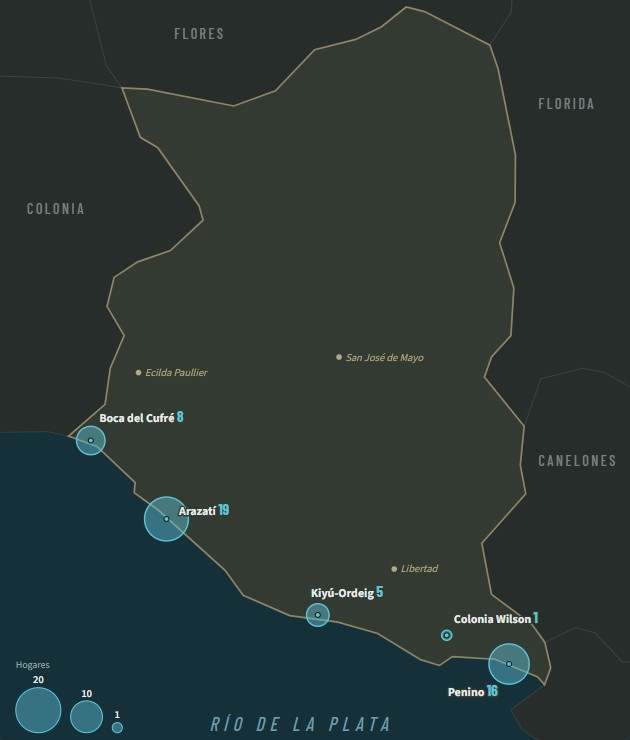
\includegraphics{hogares_localidad.jpg}

}

\caption{Distribution de hogares por localidad}

\end{figure}

\newpage

\hypertarget{viviendas}{%
\subsection{Viviendas}\label{viviendas}}

En primer lugar se podrá visualizar la forma de tenencia de los terrenos
donde están las viviendas de los hogares con personas que trabajan en la
pesca.

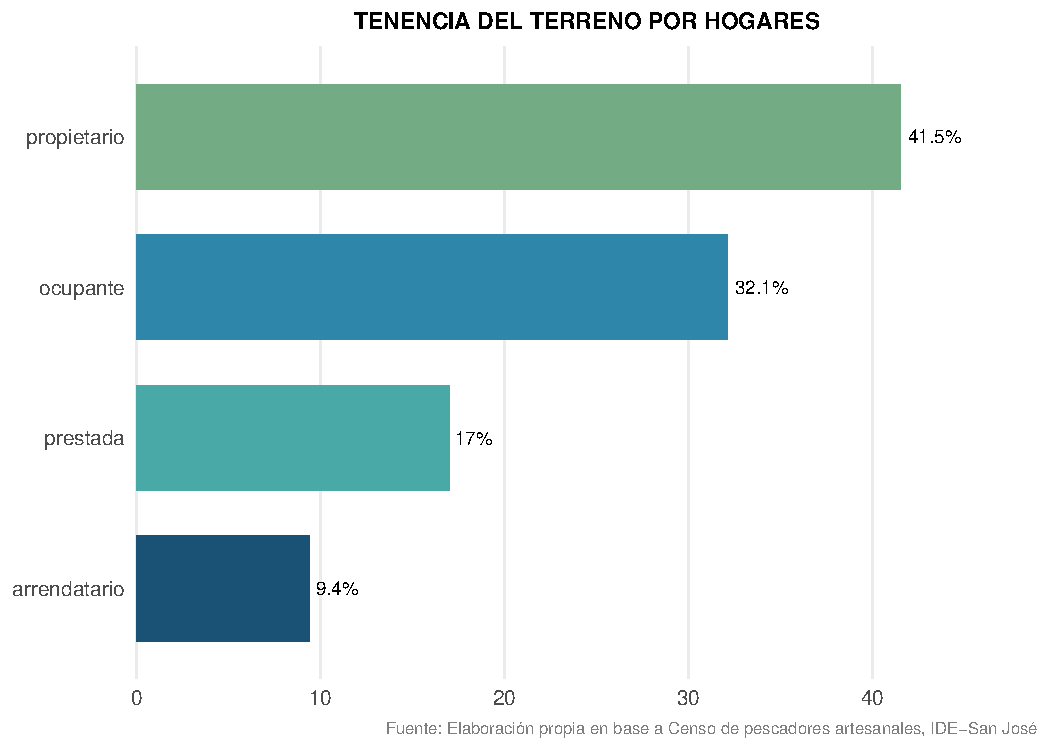
\includegraphics{analisis_pescadores_files/figure-pdf/unnamed-chunk-2-1.pdf}

Como se observa, más del 41,5\% de los hogares dicen ser propietarios
del terreno, un 32\% ocupantes, un 17\% dicen que residen sobre un
terreno prestado y un 9\% son arrendatarios. De la categoría ocupantes,
hay que señalar que el 75\% ocupan predios públicos mientras que el
resto dice estar ocupando predios privados. La mayor cantidad de
ocupantes, las dos terceras partes, están en Arazatí y Boca del Cufré.

\newpage

El gráfico siguiente muestra las condiciones de materialidad de la
vivienda de los 53 hogares de pescadores.

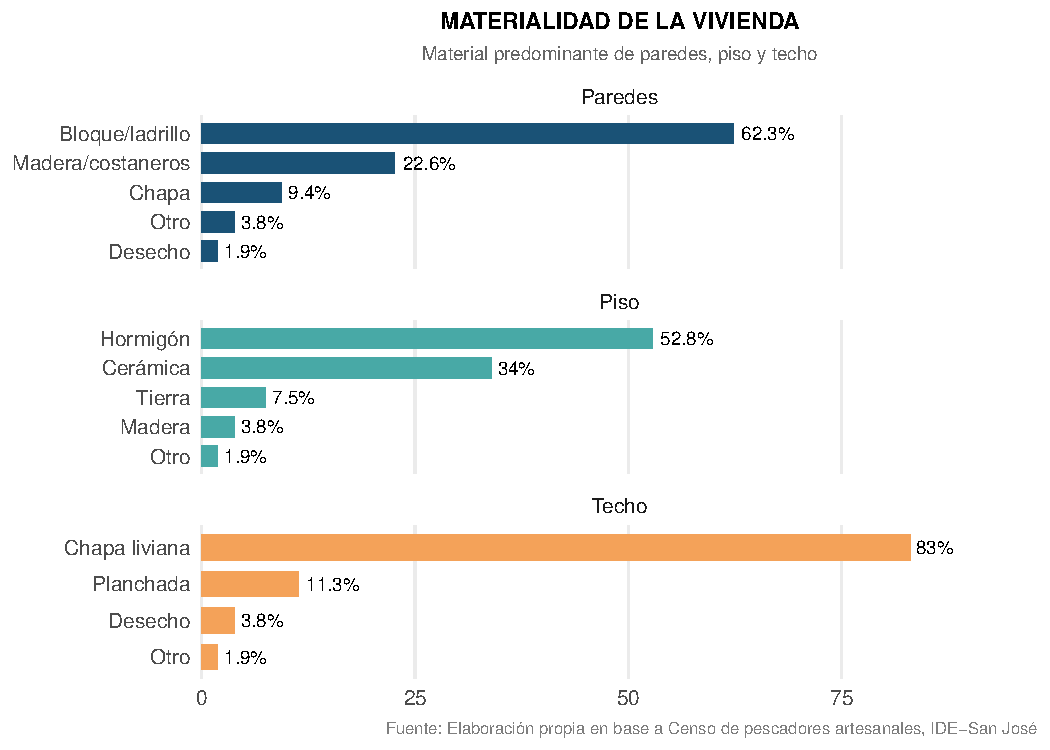
\includegraphics{analisis_pescadores_files/figure-pdf/unnamed-chunk-3-1.pdf}

Se observa que más del 62\% tienen paredes de bloque o ladrillo mientras
que el resto se describe como de materiales de menor calidad. En cuanto
a los pisos, 53\% tienen hormigón o cerámica y respecto a los techos, el
83\% son de chapa, un 11\% de planchada y un 6\% de desecho u otro. Si
se considera la materialidad de algunos de los tres componentes, se
puede observar que casi un 40\% tiene paredes con materiales precarios,
un 12\% pisos precarios y casi un 6\% techos precarios.

\newpage

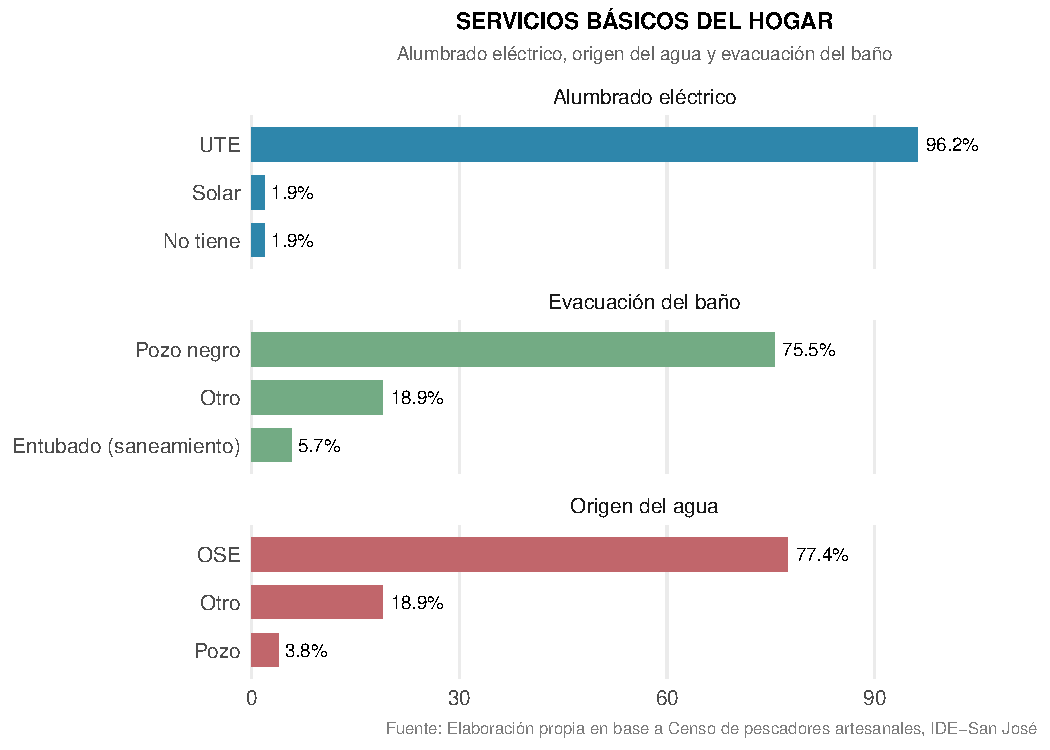
\includegraphics{analisis_pescadores_files/figure-pdf/unnamed-chunk-4-1.pdf}

En cuanto a servicios básicos, en el gráfico superior se observa que la
gran mayoría cuenta con energía eléctrica de UTE, un 2\% explota energía
solar y otro 2\% asegura no tener ninguna de estas fuentes energéticas.
La evacuación de las aguas servidas en las tres cuartas partes de los
casos se hace hacia pozo negro, casi una quinta parte a ``otro'' destino
y el 6\% a saneamiento. Con relación del agua de consumo y de uso
familiar, 77\% dice utilizar agua de OSE, una quinta parte ``otra''
fuente y un 4\% se abastece desde ``pozo''. Entre quienes dicen que se
abastecen de ``otra'' fuente, algunos entrevistados afirmaron que
recogen agua de lluvia y otros que traen en bidones o le acercan agua
familiares.

\newpage

\hypertarget{composiciuxf3n-de-los-hogares}{%
\subsection{Composición de los
hogares}\label{composiciuxf3n-de-los-hogares}}

Los hogares tienen un tamaño promedio de 3 personas, lo cual es 0,5
puntos porcentuales mayor que el tamaño promedio de los hogares
uruguayos y los del departamento.

En 37 de los hogares (70\%), la persona entrevistada convive con su
cónyuge. En dos hogares, se informó la presencia de personas con
discapacidad.

Se relevaron 14 menores de 18 años que no se encontraban escolarizados,
los cuales se encuentran en un 26,4\% del total de hogares, tal como se
aprecia en la siguiente gráfica.

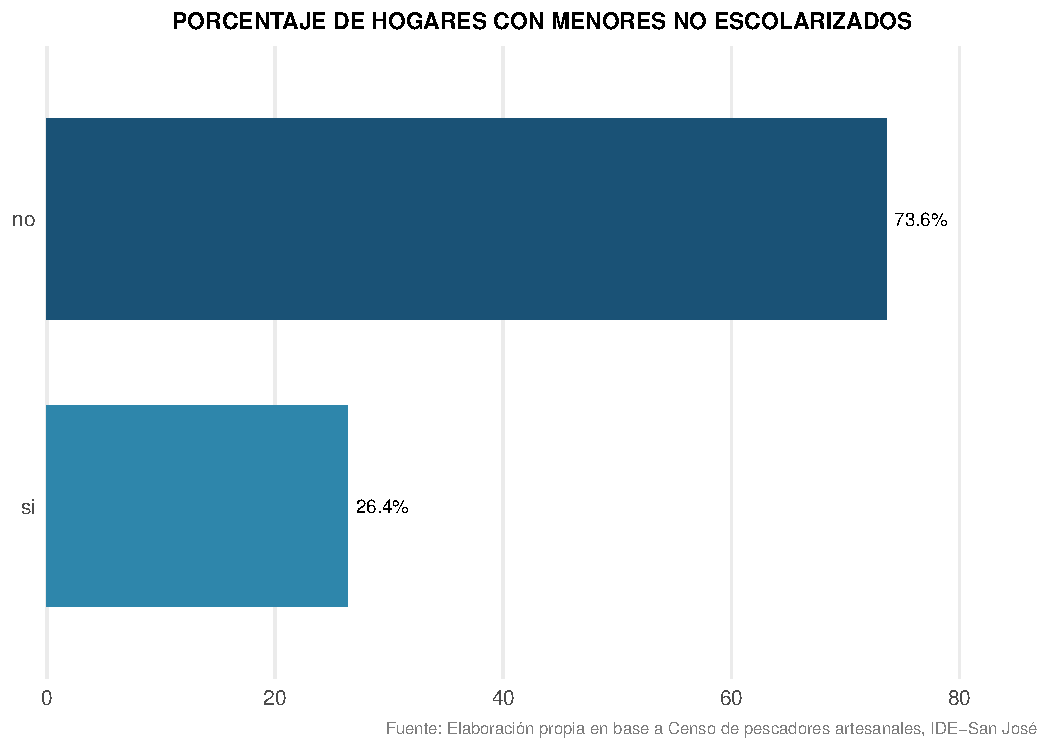
\includegraphics{analisis_pescadores_files/figure-pdf/unnamed-chunk-6-1.pdf}

\newpage

\hypertarget{caracterizaciuxf3n-demogruxe1fica-educativa-y-de-salud-de-las-personas-que-trabajan-en-la-pesca}{%
\section{Caracterización demográfica, educativa y de salud de las
personas que trabajan en la
pesca}\label{caracterizaciuxf3n-demogruxe1fica-educativa-y-de-salud-de-las-personas-que-trabajan-en-la-pesca}}

En los siguientes gráficos observamos algunas características
demográficas de las personas que declararon trabajar en la pesca
artesanal.

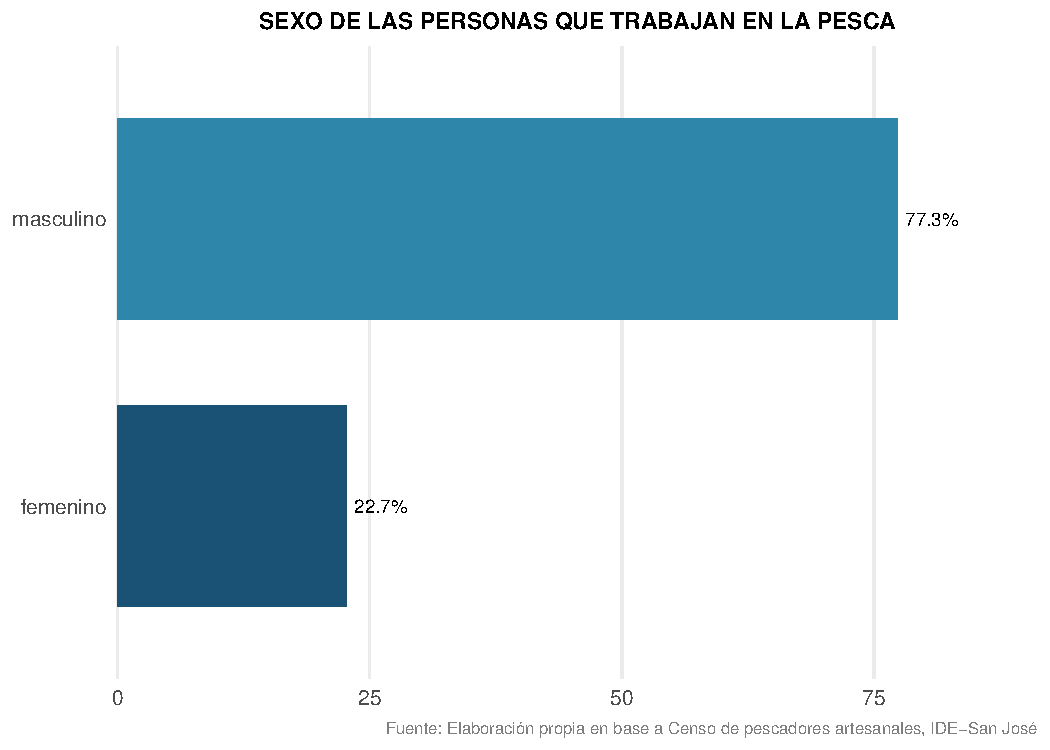
\includegraphics{analisis_pescadores_files/figure-pdf/unnamed-chunk-7-1.pdf}

El gráfico da cuenta que el 77\% son varones y el 23\% mujeres. De las
mujeres, el 70\% tienen 45 años o menos.

\newpage

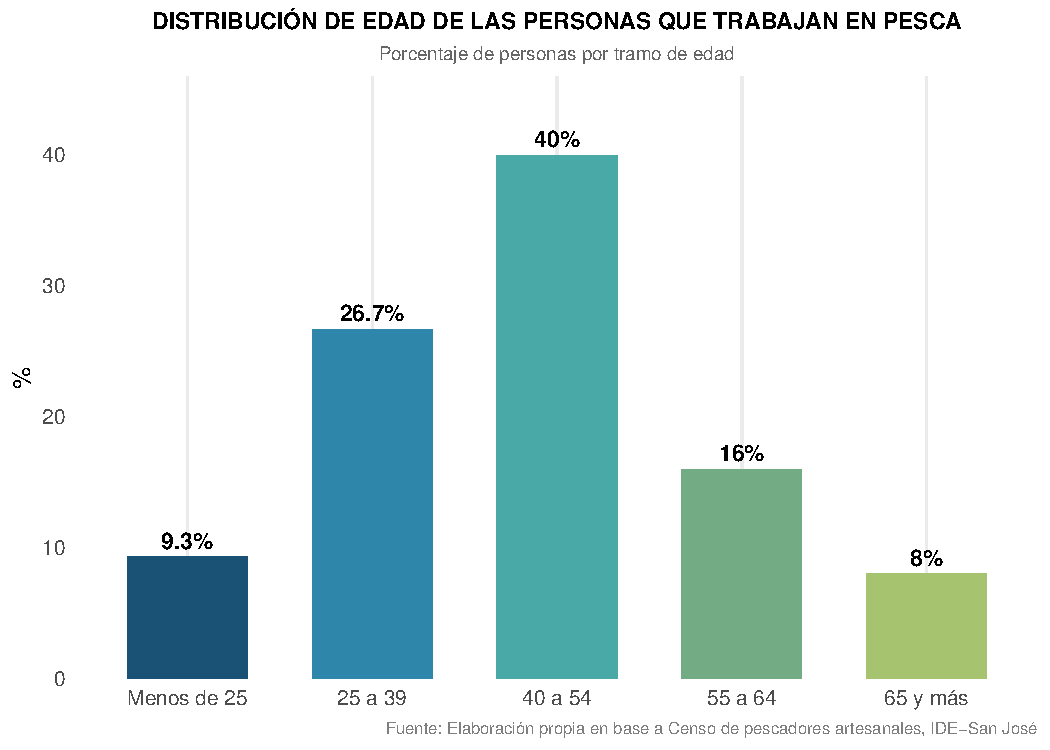
\includegraphics{analisis_pescadores_files/figure-pdf/unnamed-chunk-8-1.pdf}

Según la distribución por edades, se observa que el intervalo modal está
entre los 40 y los 54 años, grupo que representa el 40\% de los
pescadores. El 27\% está entre 25 y 39 años, el 16\% entre 55 y 64 años
y el resto se distribuye en proporciones casi iguales en los extremos de
la distribución. Resumiendo, las tres cuartas partes de los/las
pescadores/as tienen menos de 55 años.

\newpage

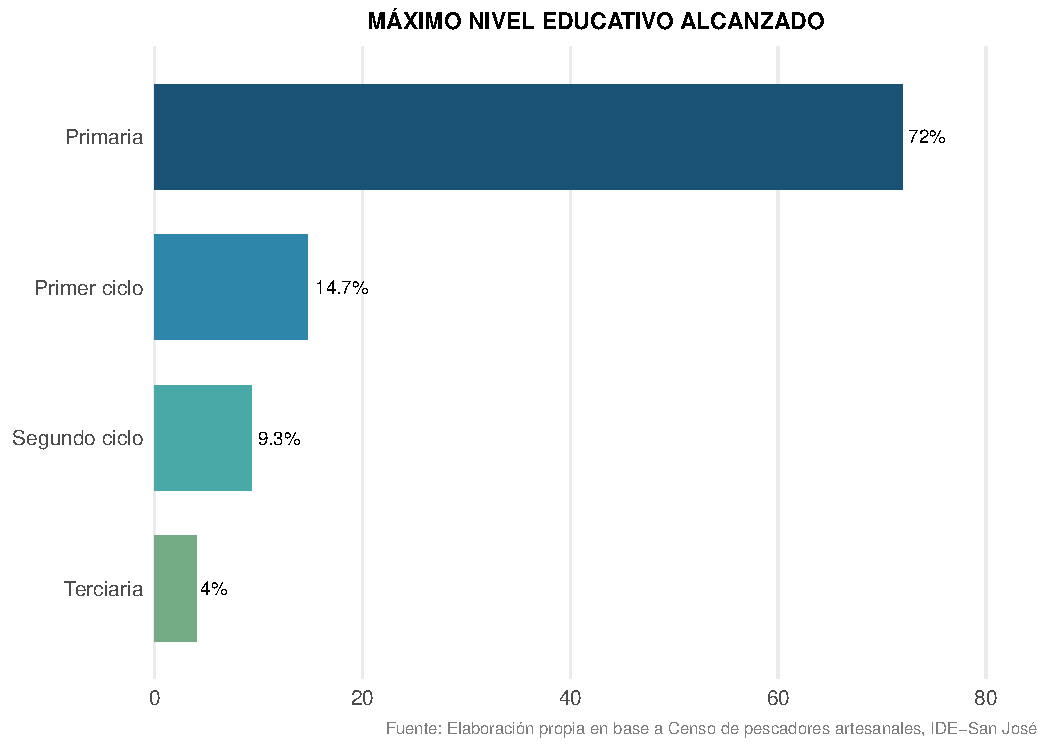
\includegraphics{analisis_pescadores_files/figure-pdf/unnamed-chunk-9-1.pdf}

Por educación formal completada, se observa que 72\% completó hasta
primaria, casi un 15\% Ciclo Básico, un 9\% alcanzó a realizar Enseñanza
Media Superior y un 4\% Educación Terciaria.

\newpage

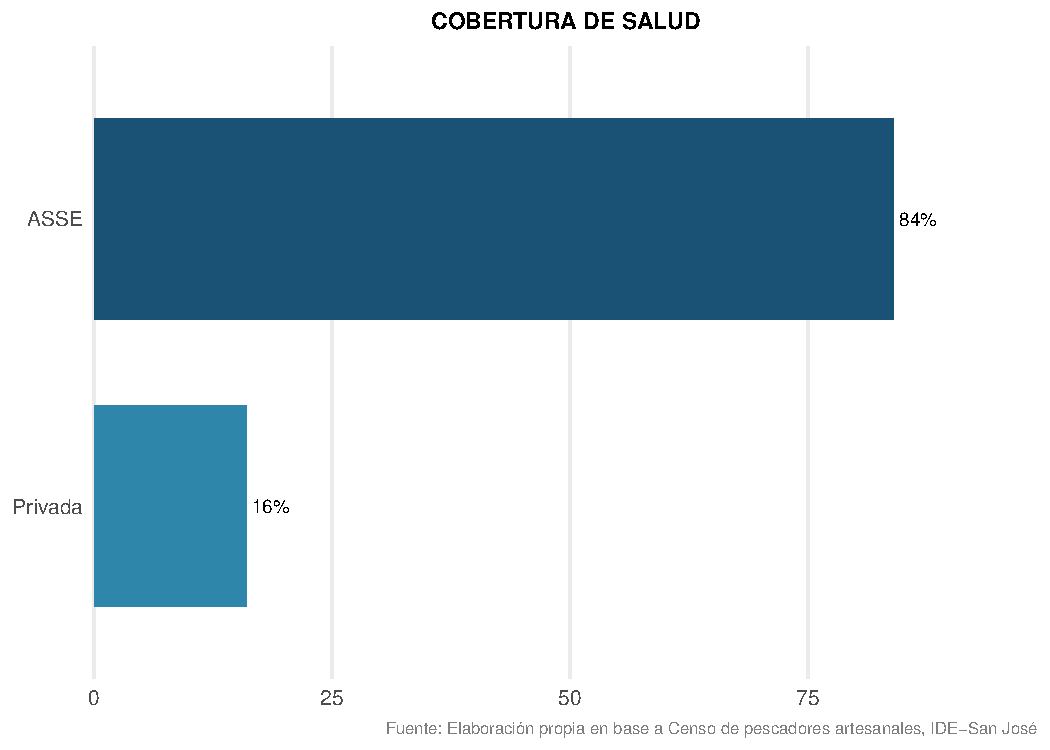
\includegraphics{analisis_pescadores_files/figure-pdf/unnamed-chunk-10-1.pdf}

En cuanto a la cobertura de salud, se constató que el 84\% se atiende en
los servicios de ASSE y un 16\% tiene cobertura privada.

\newpage

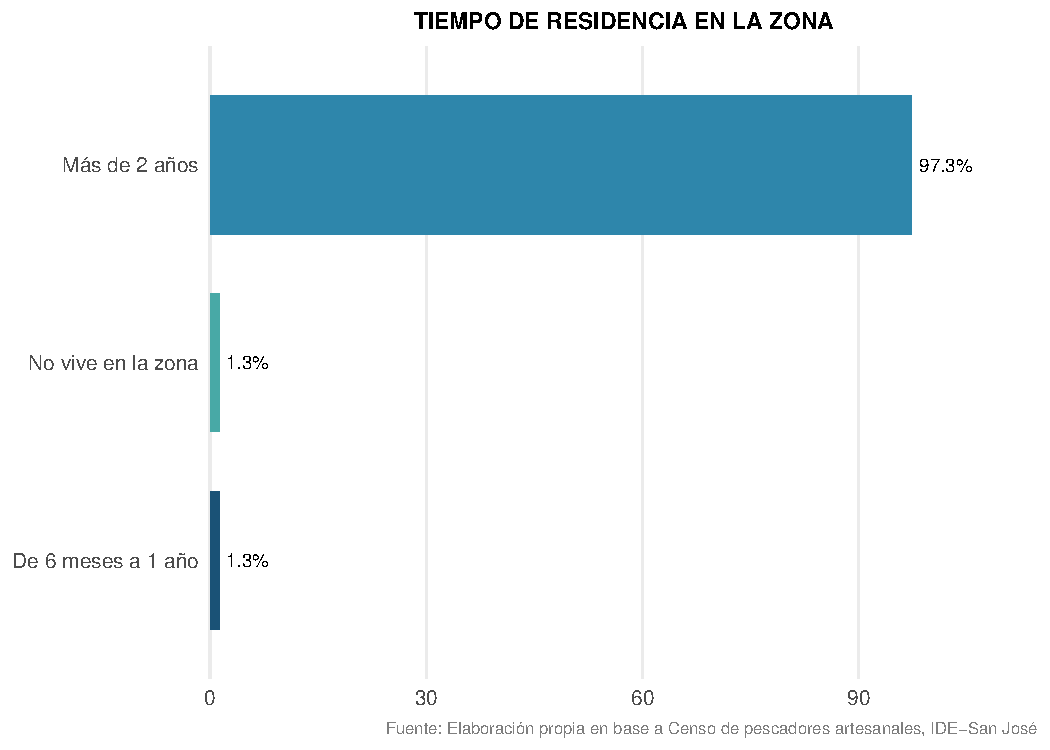
\includegraphics{analisis_pescadores_files/figure-pdf/unnamed-chunk-11-1.pdf}

En el gráfico anterior se observa la distribución porcentual por tiempo
de residencia en el lugar de trabajo. Cómo se ve, casi todos tienen un
tiempo de permanencia en sus respectivas localidades superior a los dos
años. Un 1,3\% dijo que está en el lugar hace un año o menos y un
porcentaje similar no vive en la zona donde trabaja.

\newpage

\hypertarget{actividad-pesquera}{%
\section{Actividad pesquera}\label{actividad-pesquera}}

\hypertarget{trayectoria-y-rol}{%
\subsection{Trayectoria y rol}\label{trayectoria-y-rol}}

En el siguiente gráfico se observa los años de trayectoria que tienen
los pescadores.

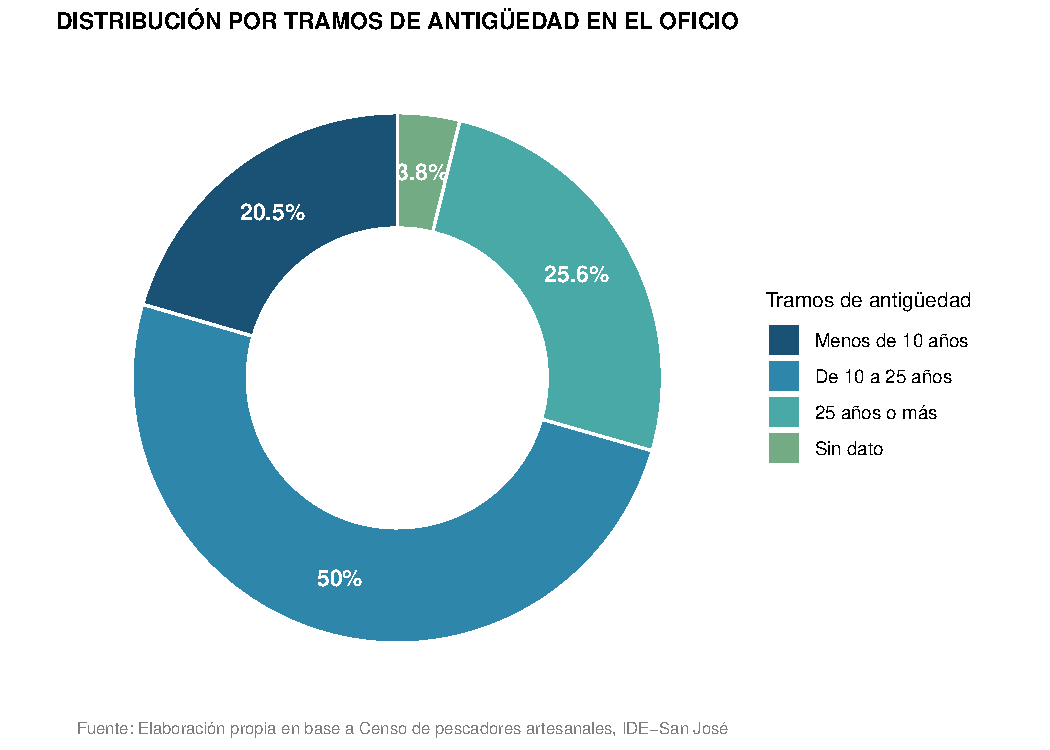
\includegraphics{analisis_pescadores_files/figure-pdf/unnamed-chunk-12-1.pdf}

Como se ve, la mitad tiene una trayectoria media en el rubro: de 10 a 25
años, la cuarta parte más de 25 años y una quinta parte, menos de 10
años. De un 4\% no se obtuvo datos.

\newpage

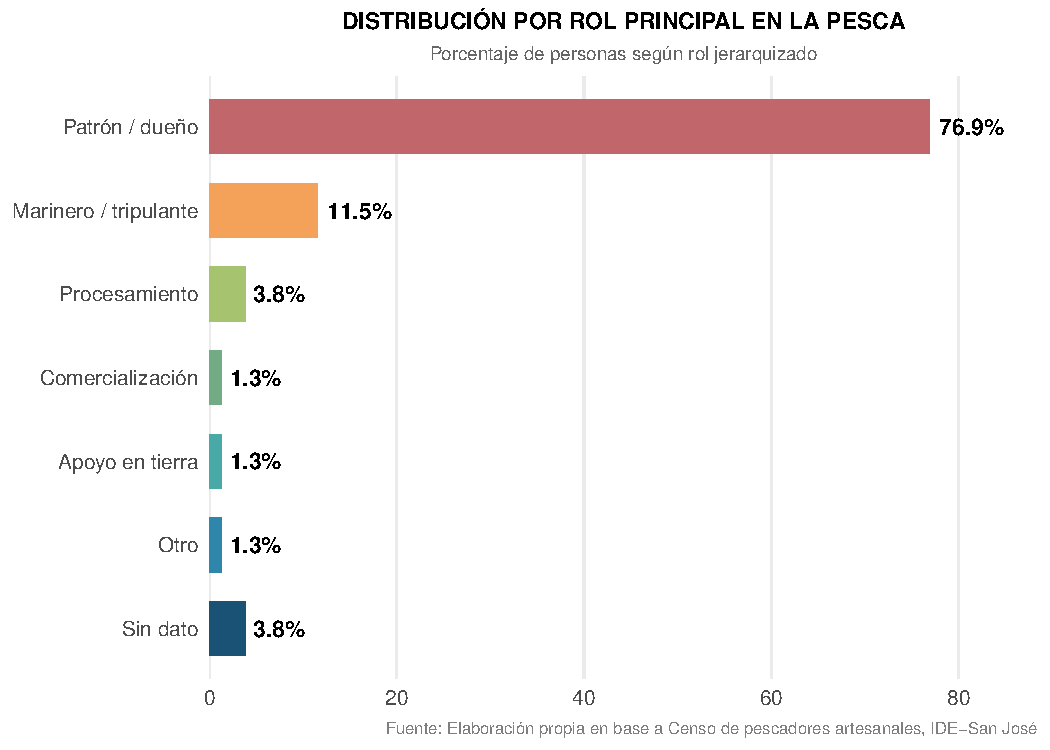
\includegraphics{analisis_pescadores_files/figure-pdf/unnamed-chunk-13-1.pdf}

En cuanto al rol en la pesca (gráfico superior), se observa que el 77\%
son patrones, un 11,5\% marineros, un 4\% trabaja en el procesamiento
del pescado y el resto se distribuye en otros roles o no sin
información.

\newpage

\hypertarget{embarcaciones-y-permisos}{%
\subsection{Embarcaciones y permisos}\label{embarcaciones-y-permisos}}

En los gráficos siguientes vemos la situación respecto a la propiedad de
las embarcaciones y la formalización de las mismas.

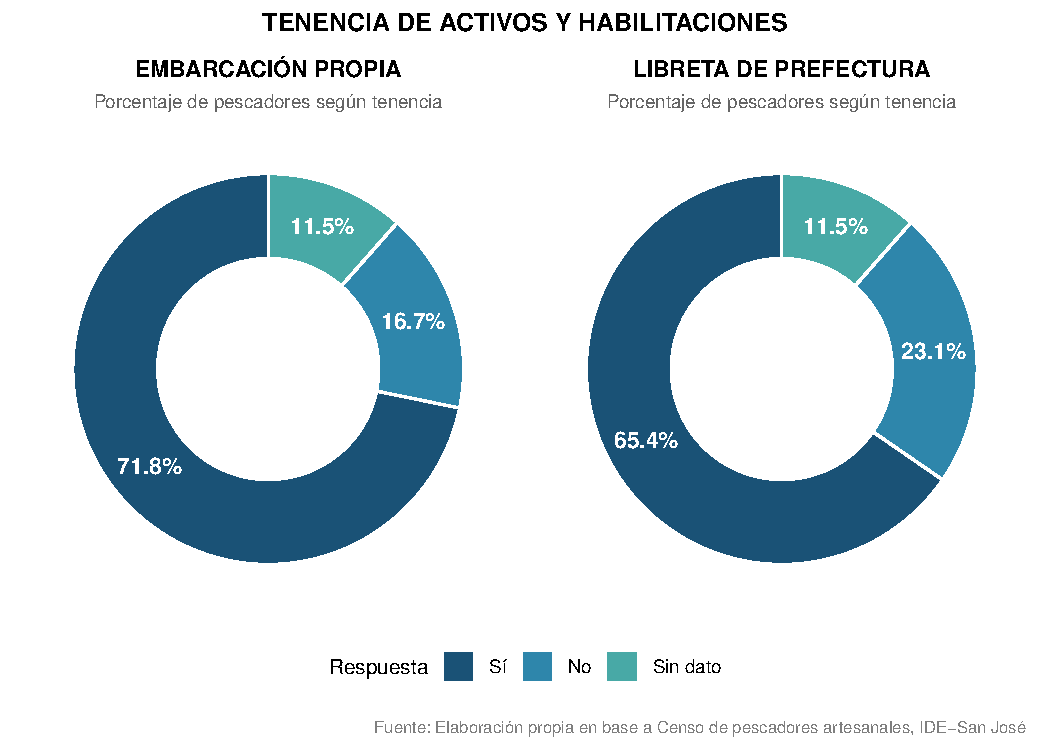
\includegraphics{analisis_pescadores_files/figure-pdf/unnamed-chunk-14-1.pdf}

En total se relevaron 62 embarcaciones. De quienes tienen embarcación
propia, la gran mayoría informó tener sólo una, excepto seis casos que
afirman tener dos cada uno

Un 72\% de las personas que trabajan en la pesca dijeron ser
propietarios de sus embarcaciones, un 17\% dijo no serlo, mientras que
un 11,5\% no informó al respecto.

En cuanto a la libreta de prefectura, un 65\% de los pescadores dijo
tenerla; casi una cuarta parte (23\%), dijo estar embarcándose sin
libreta y un 11,5\% no aportó información al respecto.

Al ser consultados si contaban con permiso de pesca se constató que un
39\% de estas embarcaciones, están trabajando sin la habilitación
correspondiente.

\newpage

\hypertarget{formalizaciuxf3n-laboral}{%
\subsection{Formalización laboral}\label{formalizaciuxf3n-laboral}}

En cuanto a la formalización laboral, la información se presenta en los
gráficos que siguen.

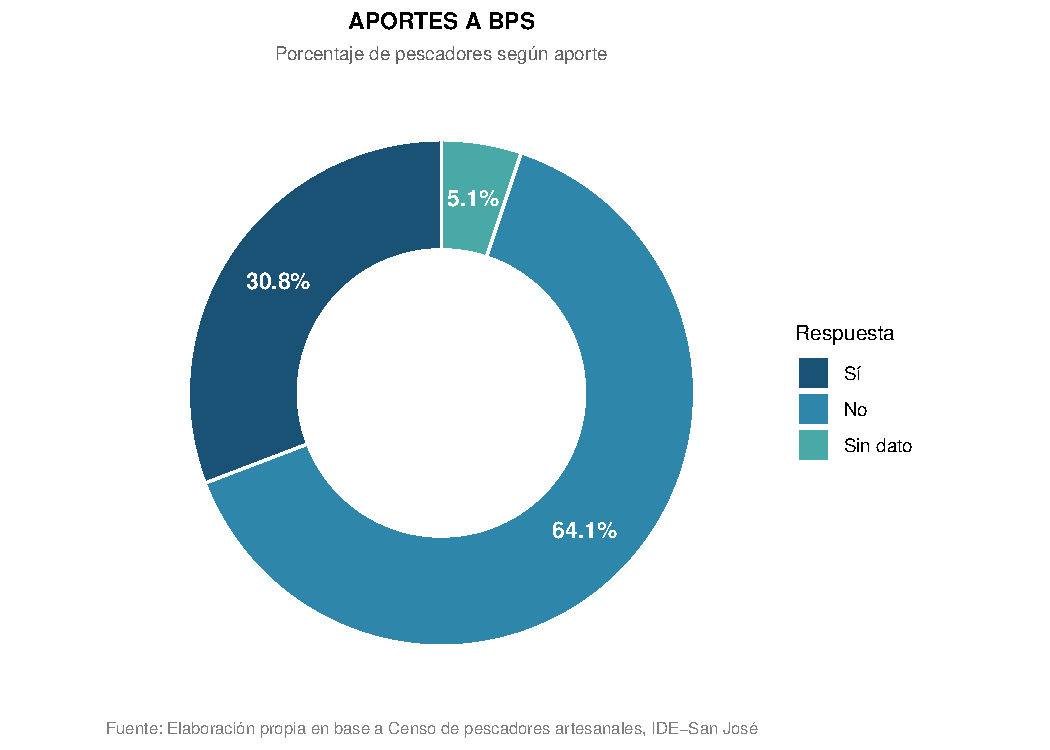
\includegraphics{analisis_pescadores_files/figure-pdf/unnamed-chunk-15-1.pdf}

Un 64\% informó que no hace aportes al BPS, un 31\% sí los hace y un 5\%
no aportó información al respecto.

Entre quienes aportan, la forma predominante es el monotributo (80\%).

\newpage

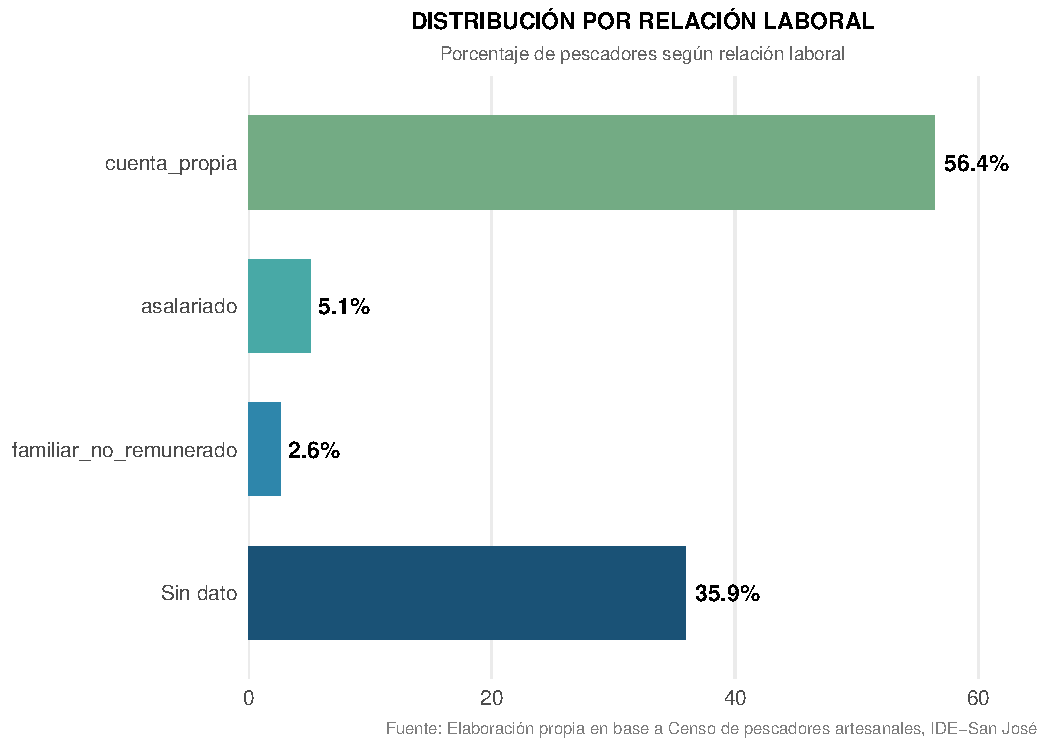
\includegraphics{analisis_pescadores_files/figure-pdf/unnamed-chunk-16-1.pdf}

En cuanto a la relación laboral, se observa que un 56\% trabajan por
cuenta propia; un 5\% son asalariados dependientes; un 3\% dicen ser
familiares no remunerados, mientras que un 36\% no aportó información al
respecto.

\newpage

\hypertarget{fuente-de-ingresos}{%
\subsection{Fuente de ingresos}\label{fuente-de-ingresos}}

En primer lugar se presentan datos sobre la continuidad laboral de los
pescadores.

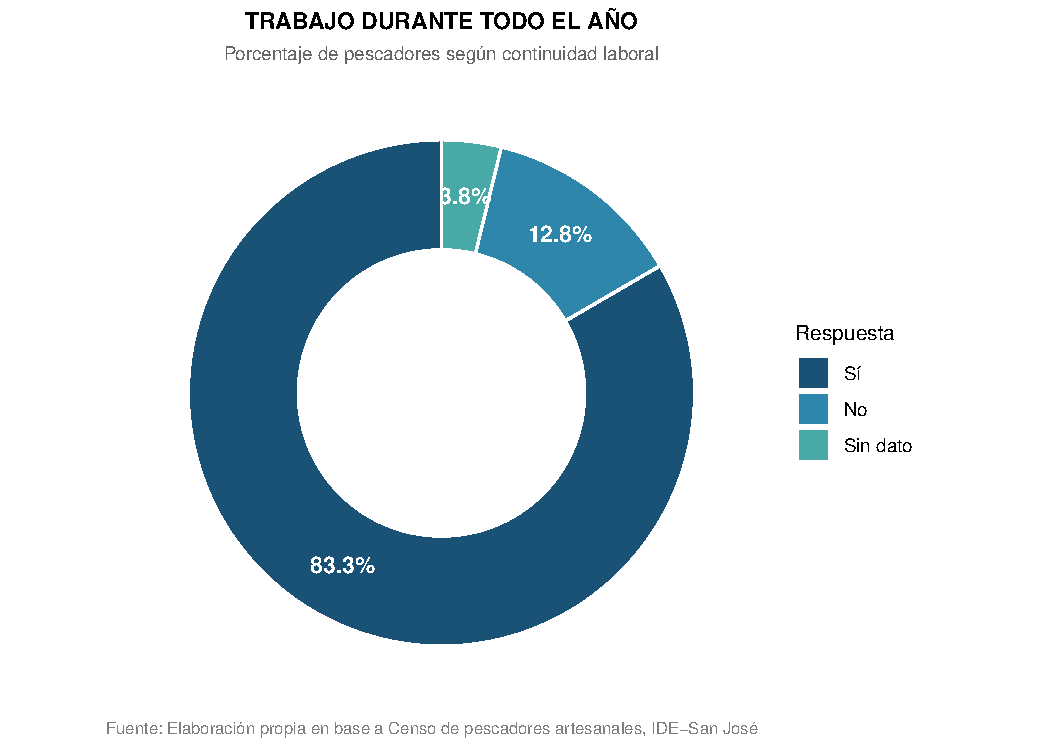
\includegraphics{analisis_pescadores_files/figure-pdf/unnamed-chunk-17-1.pdf}

En el gráfico anterior se ve que un 83\% de los pescadores dicen que
trabajan en la actividad durante todo el año, un 13\% dice que no y 4\%
no informó.

De quienes no trabajan durante todo el año, todos se concentran en
partes del segundo semestre hasta el mes de febrero.

\newpage

Respecto a la fuentes de ingresos se presentan los siguientes datos.

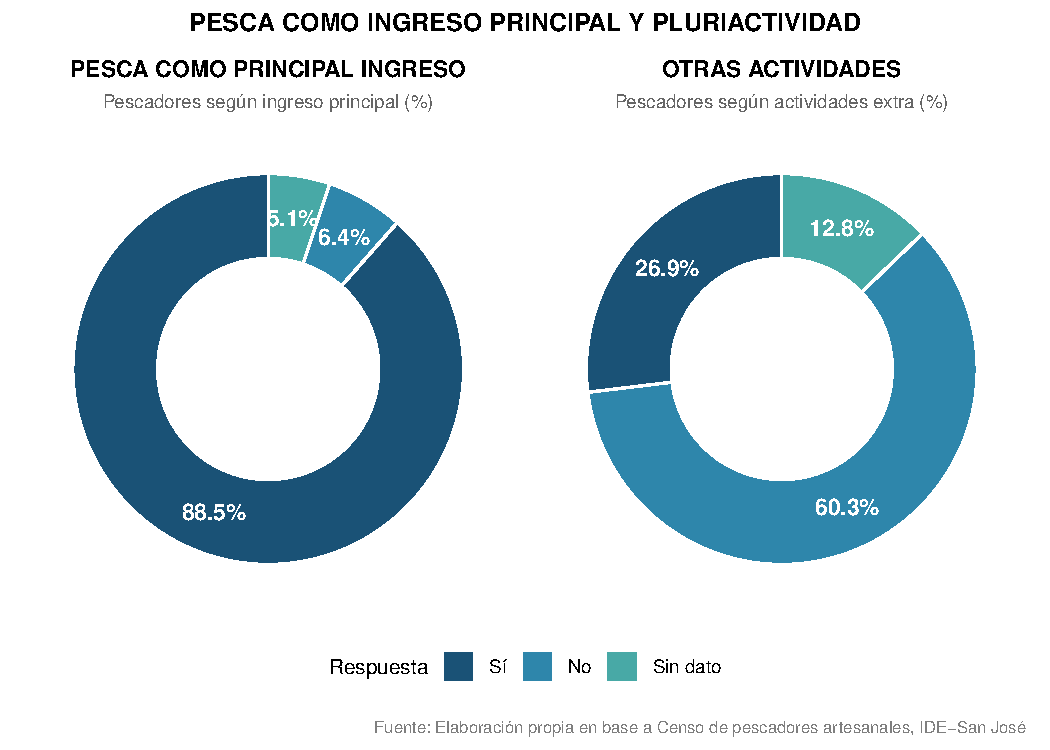
\includegraphics{analisis_pescadores_files/figure-pdf/unnamed-chunk-18-1.pdf}

El 88,5\% de los que trabajan en la pesca aseguró que su principal
fuente de ingreso es la pesca, un 6\% dijo que su ingreso principal
provenía de otra actividad y el resto no dio información.

A su vez, un 27\% de las personas que trabajan en la pesca afirmaron que
realizan otras actividades complementarias. Las cuales se concentran en
albañilería y changas, seguidas por trabajos rurales y, en menor medida,
ocupaciones diversas como limpieza, gastronomía, almacén y leña. La
presencia de respuestas múltiples evidencia una marcada pluriactividad
entre los pescadores.

\newpage

En el gráfico siguiente se observa, la distribución de los intervalos de
ingreso (ganancia resultante una vez pagado todos los costos), según
zafra y fuera de zafra de acuerdo a lo que marcan los pescadores.

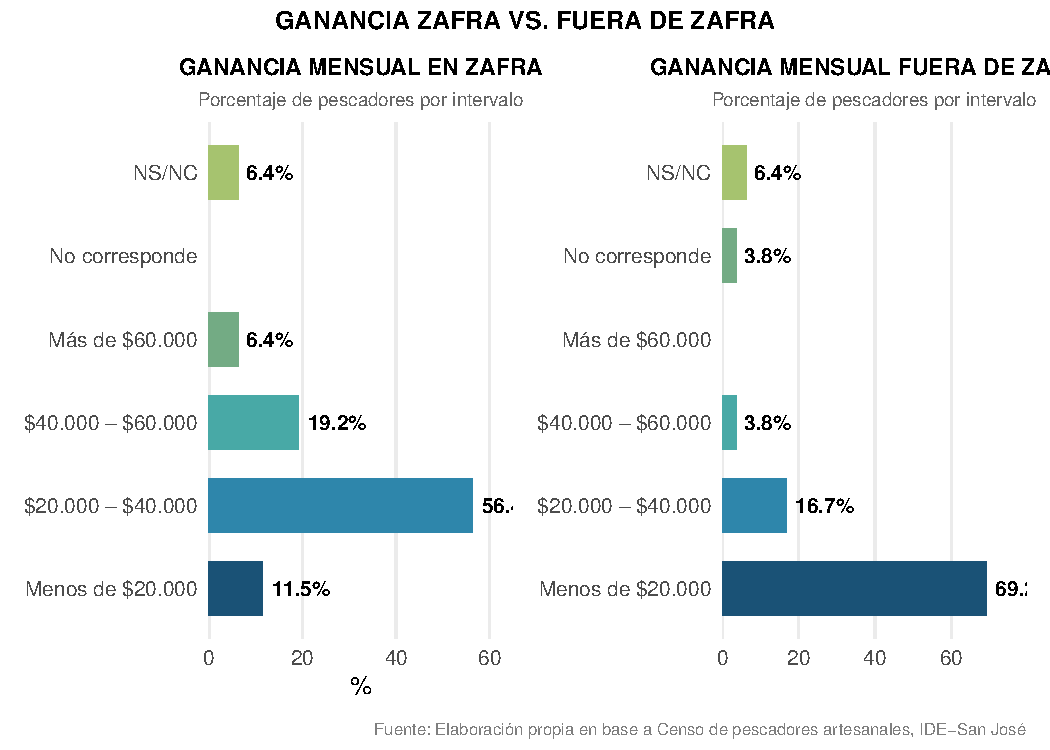
\includegraphics{analisis_pescadores_files/figure-pdf/unnamed-chunk-19-1.pdf}

En zafra, la mayoría, el 56\%, dijo tener una ganancia de entre 20.000 y
40.000 pesos. El resto se distribuyó así: una quinta parte entre 40.000
y 60.000, un 6\% afirmó ganar más de 60.000 pesos y un 11,5\% dijo ganar
menos de 20.000 pesos; más de 6\% no respondió a esta pregunta.

Fuera de zafra, más de las dos terceras parte, aseguró que ganaba menos
de 20.000 pesos; un 17\% entre 20.000 y 40.000 y un 4\%, entre 40.000 y
60.000 pesos.

\newpage

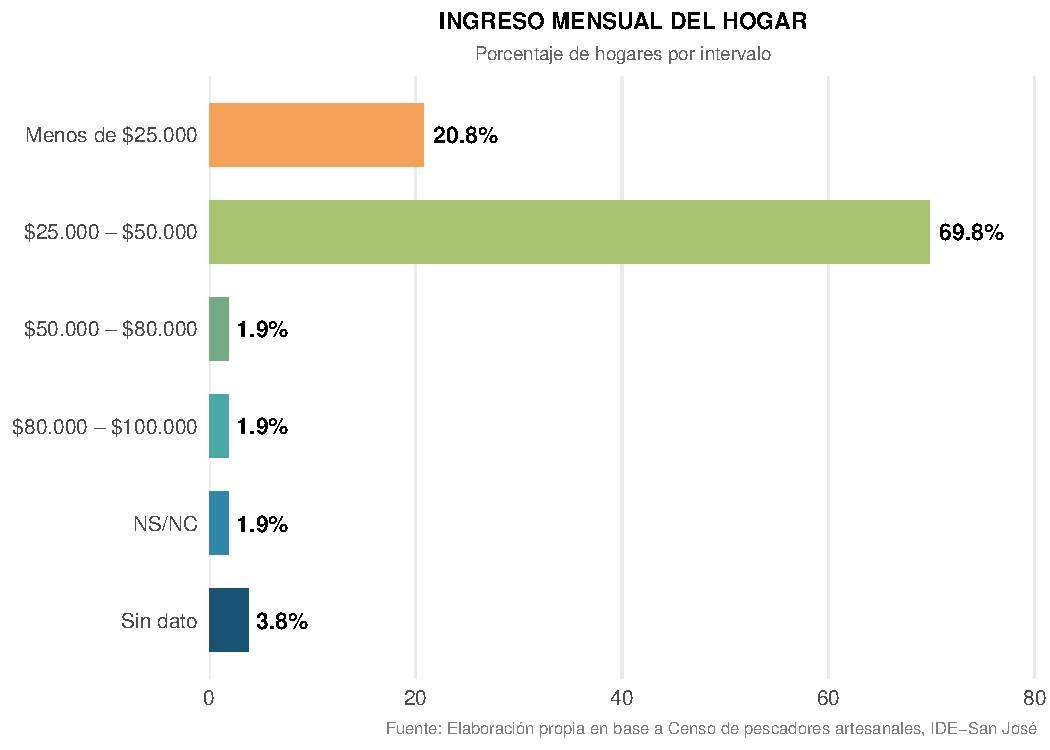
\includegraphics{analisis_pescadores_files/figure-pdf/unnamed-chunk-20-1.pdf}

En cuanto al ingreso del hogar, el 70\% informó que el mismo estaba
entre 25.000 y 50.000 pesos, un 21\% dijo que tenían un ingreso menor a
25.000 pesos, casi un 4\% supera los \$50.000 y un 6\% no aportó
información al respecto.

\newpage

\hypertarget{capacitaciuxf3n-organizaciuxf3n-y-percepciuxf3n-del-sector}{%
\subsection{Capacitación, organización y percepción del
sector}\label{capacitaciuxf3n-organizaciuxf3n-y-percepciuxf3n-del-sector}}

Se preguntó a los pescadores, qué interés tenían en recibir alguna
capacitación y otros aspectos referidos a organización, participación de
instancias colectivas y percepción de problemas del sector.

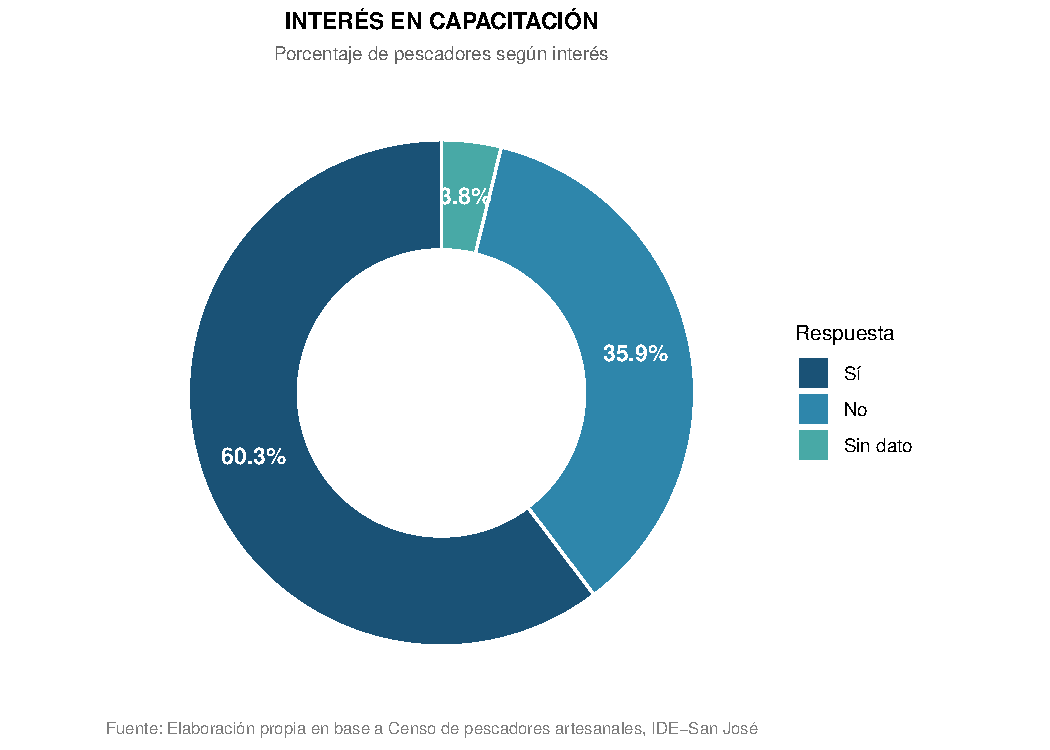
\includegraphics{analisis_pescadores_files/figure-pdf/unnamed-chunk-21-1.pdf}

Un 60\% respondió tener interés en recibir capacitaciones, un 36\% dijo
no estar interesado y un 4\% no informó al respecto.

\newpage

A los interesados en recibir capacitaciones, se les indicó que podían
elegir hasta tres de un menú de opciones ya establecido.

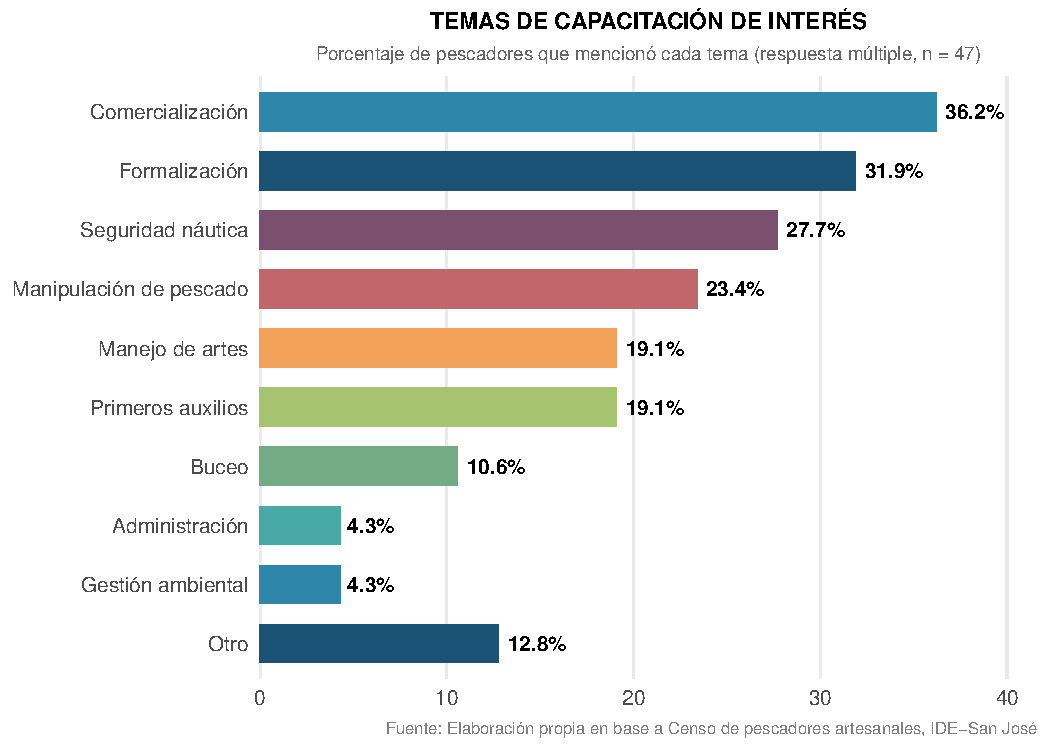
\includegraphics{analisis_pescadores_files/figure-pdf/unnamed-chunk-22-1.pdf}

El tema más mencionado fue comercialización, elegido por el 36\% de los
pescadores; en segundo lugar formalización, mencionado por el 32\%; en
tercer lugar, 28\%, el interés se volcó por seguridad naútica y en
cuarto lugar, manipulación del pescado, mencionado por el 23\% de los
pescadores. También otros temas como manejo de artes de pesca y primeros
auxilios fueron mencionados por casi una quinta parte de los entrevistas
como temas de interés para capacitarse. Con porcentajes menores de
menciones aparecen buceo, administración y gestión ambiental. En
``Otro'' se encuentran tres menciones más a ``Administración'', una a
``Meteorología'' y otra a ``Mecánica''.

\newpage

En cuanto a la participación en asociaciones o organizaciones sociales
por parte de los pescadores, solamente se encuentran dos casos que
declaran participar de sindicatos, mostrando un bajo nivel asociativo
del sector.

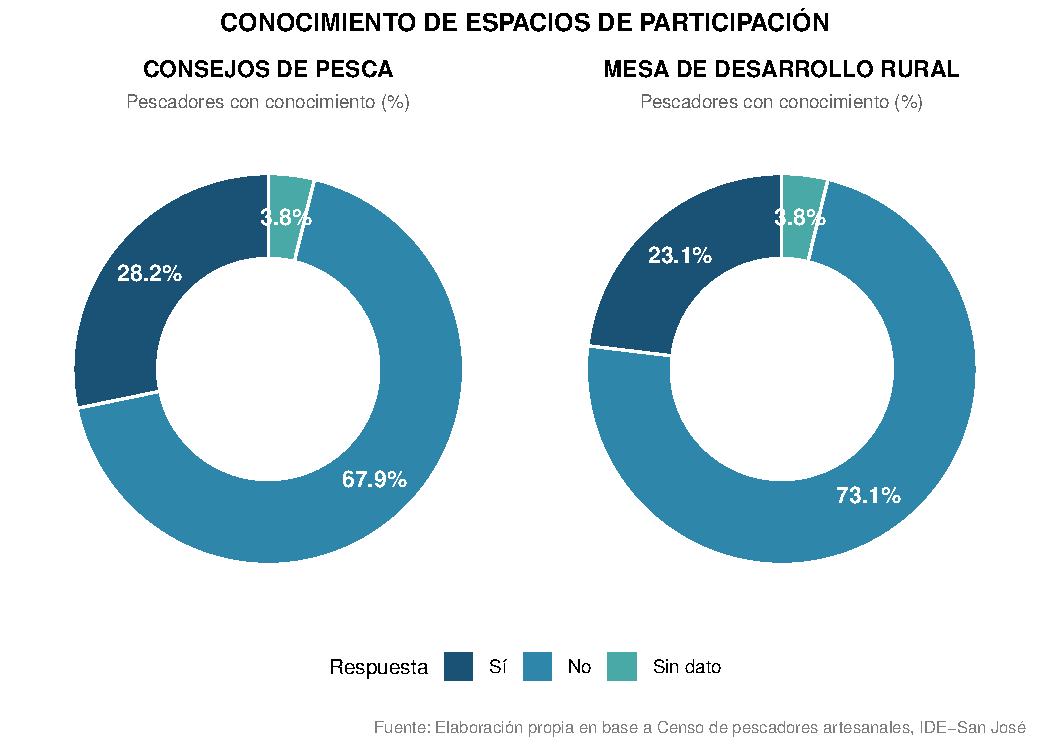
\includegraphics{analisis_pescadores_files/figure-pdf/unnamed-chunk-23-1.pdf}

Se preguntó en particular qué conocimiento tenían sobre dos ámbitos de
participación: Consejos de Pesca y Mesa de Desarrollo Rural. Como vemos
la gran mayoría desconoce ambos espacios: el 70\% y el 73\%
respectivamente. Un 28\% conoce los Consejos de Pesca y un 23\% la Mesa
de Desarrollo Rural. Adentrándonos en detalles sobre estos últimos, sólo
la quinta parte de los que conocen no encuentra útil la participación en
estos espacios.

\newpage

Se pidió a los pescadores que señalaran cuáles son problemas que
enfrenta el sector. Para ello se les entregó una tarjeta que contenía un
listado de posibles dificultades y se les solicitó que seleccionaran
hasta tres.

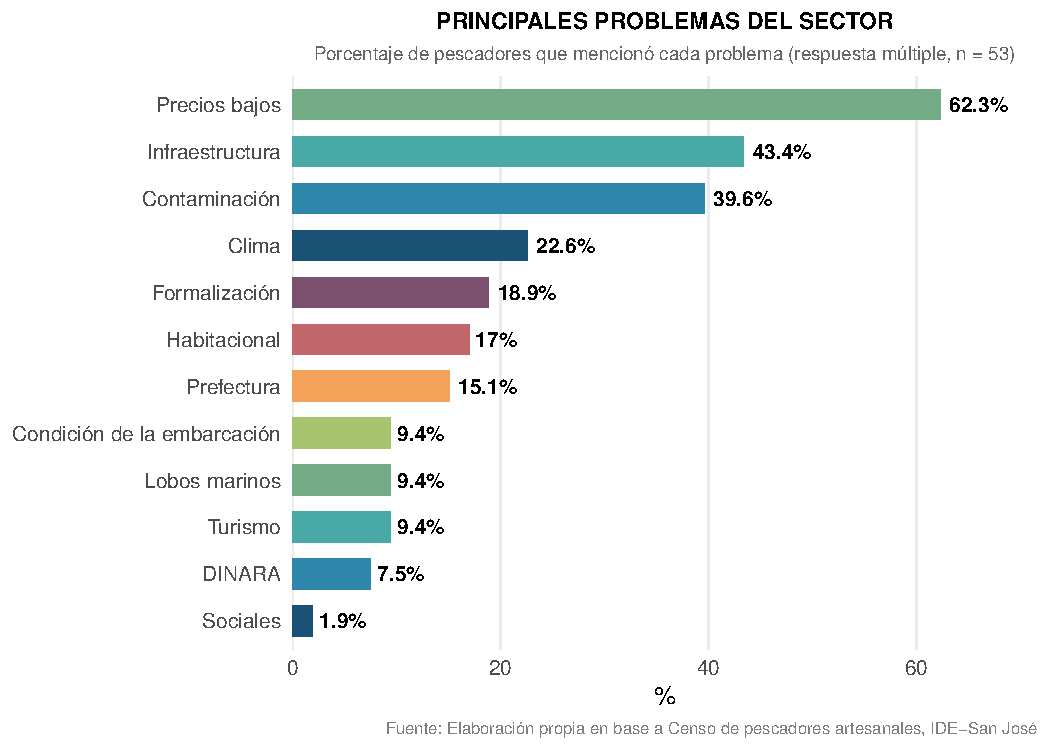
\includegraphics{analisis_pescadores_files/figure-pdf/unnamed-chunk-24-1.pdf}

Como se observa en el gráfico anterior, el 62\% de los pescadores
mencionó precios bajos, un 43\% marcó infraestructura, un 40\%
contaminación. Porcentajes menores pero también significativos
mencionaron como problemas aspectos relativos al clima, la
formalización, dificultades de vivienda y problemas con prefectura.
Menos del 10\% de los pescadores, también mencionaron ``condición de la
embarcación'', la presencia de ``lobos marinos'' y conflictos con la
actividad turística.

\newpage

En la pregunta siguiente se solicitó a cada pescador, que de los tres
problemas identificados, seleccionara aquel que considerara prioritario
por lo que este gráfico suma 100.

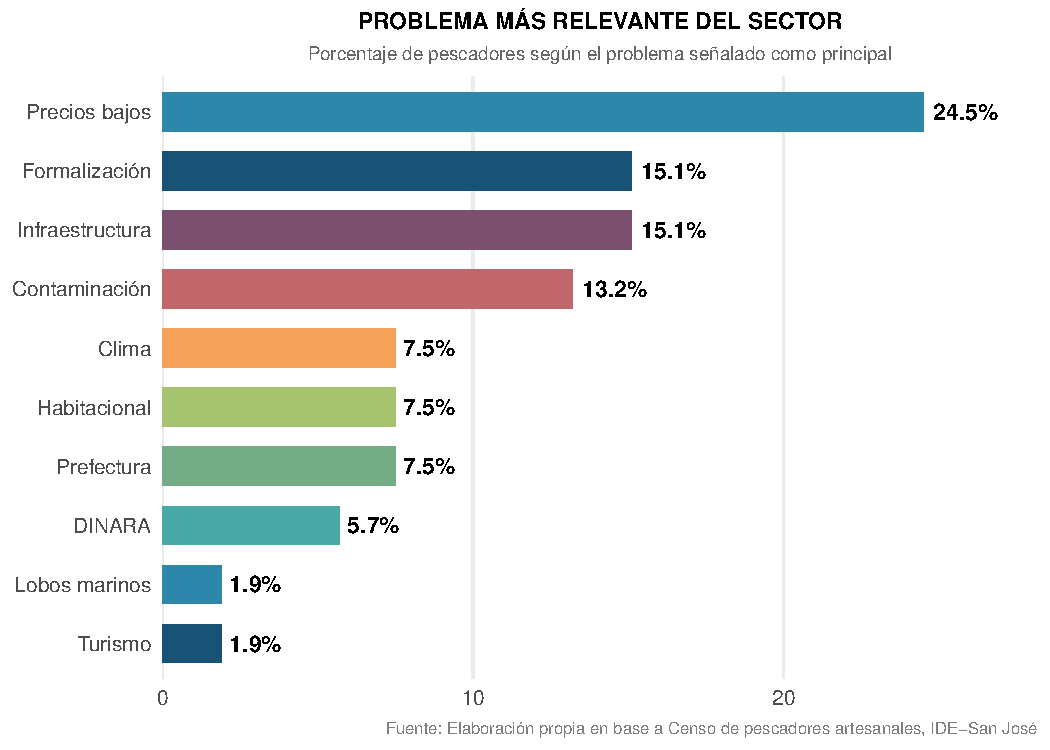
\includegraphics{analisis_pescadores_files/figure-pdf/unnamed-chunk-25-1.pdf}

La cuarta parte, sostuvo que el problema principal es el relativo a los
bajos precios, un 15\% jerarquizó el tema de la formalización y un
porcentaje igual problemas de infraestructura. Un 13\% seleccionó como
problema principal el derivado de la contaminación y luego aparecen en
ese orden temas tales como clima, vivienda y prefectura con 7,5\%;
Dinara con 6\% de los pescadores que la mencionan como fuente de
problema y lobos marinos y turismo con 2\% cada uno.

\newpage

Para cada uno de los problemas jerarquizados se preguntó a los
pescadores que solución darían. A continuación se presenta un análisis
descriptivo de lo recabado.

\emph{Intermediación y comercialización.}

Los pescadores identifican a los intermediarios como el principal
eslabón que captura el valor de su trabajo, y proponen tanto eliminarlos
como buscar canales alternativos: ``Sacar los intermediarios''; ``Buscar
mejores mercados para mejorar precios''; ``Intervención del Estado, hay
un monopolio: (mencionan empresa) Oligopolio. Asimetría porque tienen
muchas barcas.''

\emph{Precio y rentabilidad.}

Directamente vinculado al punto anterior, aparece el reclamo por mejores
precios y estabilidad ``Que sepa, hace años se paga lo mismo'';
``Estabilidad en el precio'';``Costos suben''

\emph{Formalización y trámites.}

Una demanda recurrente es simplificar los procedimientos y mejorar el
acceso a la información, sin perder de vista la necesidad de regularizar
la actividad: ``Simplificar para permiso, menos vueltas'';``Más rápido
los trámites, y más información'';``Abrir ventanilla''

\emph{Infraestructura.}

Las propuestas se orientan a obras concretas que mejoren las condiciones
de trabajo: muelles, caminería, accesos y servicios básicos: ``Construir
un muelle''; ``Agua para consumo y muelle'';``Mejora de entrada,
hormigón''

\emph{Control ambiental.}

Frente a la contaminación, las soluciones apuntan a mayor fiscalización
y a responsabilizar a todos los actores, no solo a los pescadores:
``Control agroquímicos de los campos o prohibición''; ``Tachos, para los
restos de los pescados''; ``Que la gente de las cámaras de frío no tiren
el pescado, no son los pescadores que tiran al arroyo''.

\emph{Control y fiscalización.}

Algunas respuestas se centran en mejorar y equiparar el control de la
actividad: ``Que se pueda hacer registros cerca y control parejo para
todas las embarcaciones''; ``Mejorar el control''.

\emph{Vivienda e ingreso.}

Aparecen demandas vinculadas a las condiciones de vida: ``Alguna
vivienda, para dejar de pagar alquiler'';``Apoyo de
materiales'';``Teniendo dinero para comprar.''

\emph{Gestión con DINARA.}

Se mencionan facilidades para la formalización y la necesidad de
permisos accesibles: ``Que den más facilidades para la formalización'';
``Falta de facilidades para la formalización''.

\emph{Convivencia con turismo y fauna.}

Respuestas puntuales pero significativas por su contenido simbólico:
``Respetar el espacio de trabajo''(turismo); ``No hay, es el hábitat de
ellos también'' (lobos marinos)

\textbf{Tres ejes ordenan el conjunto de las propuestas:}

\begin{enumerate}
\def\labelenumi{\arabic{enumi}.}
\item
  Eje económico-comercial (intermediación, precio): el problema más
  sentido y el que más soluciones concentra. El reclamo apunta a romper
  la asimetría de poder en la cadena de comercialización.
\item
  Eje institucional-regulatorio (formalización, DINARA, prefectura):
  convive una doble demanda: simplificar los trámites y mejorar el
  control de la actividad, lo que sugiere que el problema no es la
  regulación en sí, sino cómo se implementa.
\item
  Eje territorial-ambiental (infraestructura, contaminación, turismo):
  las soluciones son concretas y localizadas, y expresan una
  preocupación por las condiciones materiales del trabajo y por el
  cuidado del ambiente del que depende la actividad.
\end{enumerate}

\newpage

Finalmente se pregunta a los pescadores qué es lo que más valoran de su
profesión. Se presenta un análisis al respecto.

\emph{Eje 1 --- Autonomía e independencia}

Es, sin duda, el valor más mencionado. Aparece bajo distintas
formulaciones que remiten a la misma idea: la posibilidad de organizar
el propio trabajo, no tener jefe, decidir cuándo y cómo salir a
pescar.Lo expresan así: ``Ser independiente''; ``Trabajar para mí mismo,
libertad''; ``Trabajo independiente''; ``Ser libre de tu vida'' La
independencia aquí no es solo una condición laboral: es un valor
identitario, lo que define al oficio frente a otras ocupaciones.

\emph{Eje 2 --- Libertad y tranquilidad}

Estrechamente ligado al anterior, pero con un matiz más emocional y
existencial. Aparecen dos palabras que se repiten una y otra vez:
libertad y tranquilidad. De esta manera: ``Libertad''; ``Tranquilidad'';
``Paz y tranquilidad''; ``Tranquilidad y libertad''.Es llamativo el peso
de estos términos, casi como un estribillo que atraviesa las respuestas.
Sugiere que el oficio ofrece algo que va más allá del ingreso: un modo
de vida asociado al ritmo propio, al contacto con el entorno y a la
ausencia de presiones externas.

\emph{Eje 3 --- Gusto por la actividad y vínculo con la naturaleza}

Muchos pescadores valoran simplemente hacer lo que les gusta, con un
vínculo explícito con el entorno natural: ``Me gusta pescar''; ``Es lo
que me gusta y puedo vivir''; ``La naturaleza'';``El entorno con la
naturaleza.'' Este eje combina vocación (hacer lo que a uno le gusta) y
pertenencia territorial (el río, el mar, el entorno como parte del
trabajo).

\emph{Eje 4 --- Ser patrón y sostener el ingreso}

Un grupo importante menciona el valor de ser patrón (tener embarcación
propia) y de poder vivir de la pesca: ``Ser patrón'';``El ser patrón'';
``Poder vivir de la pesca''; ``El ingreso''; ``Que hay trabajo y comida
todos los días''.Acá la valoración es material y de estatus: no se trata
solo de libertad, sino de autonomía económica y de ser dueño de los
medios de producción.

\emph{Eje 5 --- El oficio como forma de vida}

Algunas respuestas sintetizan todo lo anterior y expresan que la pesca
no es solo un trabajo, sino una forma de vida: ``Es la forma de vida'';
``Que es la forma de vivir'';``El arte como tal''. Es la formulación más
densa simbólicamente: el oficio como identidad, no como ocupación
transitoria.

\emph{Menciones negativas o ambivalentes}

Hay dos respuestas que rompen el tono positivo general y merecen
señalarse aparte: ``No, que es sacrificado'';``Sacrificio''. Estas voces
introducen el costo físico y personal del oficio, y son importantes para
no romantizar el análisis: la libertad y la tranquilidad conviven con un
trabajo duro, incierto y expuesto a condiciones adversas.

\emph{Lectura transversal}

Tres ideas ordenan el conjunto:

\begin{itemize}
\item
  Autonomía como núcleo identitario: ser independiente, ser patrón,
  trabajar para uno mismo. Es lo que distingue a la pesca de un empleo
  asalariado.
\item
  Bienestar subjetivo: libertad, tranquilidad, paz. No es solo una
  libertad formal, es una experiencia cotidiana de vivir sin presiones
  externas.
\item
  Vocación y pertenencia: gusto por la actividad y vínculo con el
  entorno natural y el territorio.
\end{itemize}

Por último, se recaban algunas observaciones generales, donde vale la
pena destacar las menciones a la merma percibida sobre la cantidad de
pescado en los últimos 5 años, el mal estado de la bajadas en varios
puntos y lo díficil que resulta mantener el monotributo fuera de zafra.

\newpage

\hypertarget{embarcaciones}{%
\section{Embarcaciones}\label{embarcaciones}}

En este apartado, se incorpora el análisis de la pesca artesanal del
departamento de San José por las embarcaciones.

En este capítulo se tiene información de 60 embarcaciones, dos menos de
las que fueran informadas en la primera enumeración por los pescadores
entrevistados.

A continuación vemos los puertos bases de las embarcaciones relevadas.

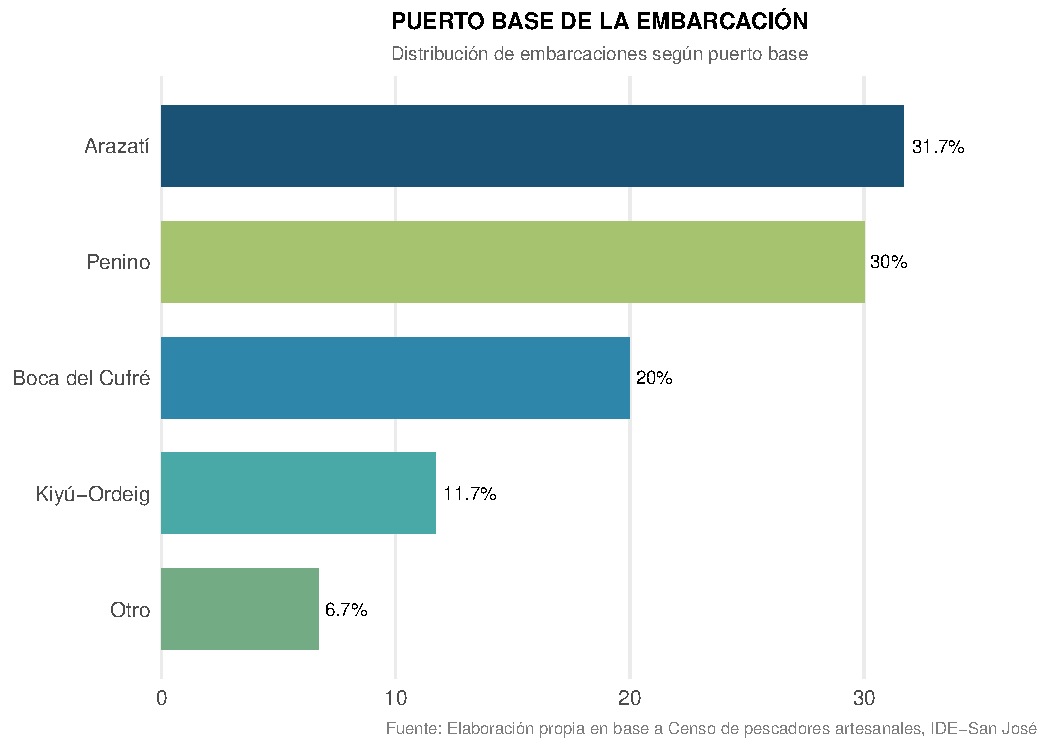
\includegraphics{analisis_pescadores_files/figure-pdf/unnamed-chunk-26-1.pdf}

En el gráfico superior se observa que el puerto base que tiene más
embarcaciones es Arazatí con el 32\% de las mismas y, en segundo lugar,
Penino, con el 30\%. Es decir que estos dos puertos base, concentran el
62\% de las embarcaciones que operan en la pesca artesanal de la costa
platense de San José. Después vemos que el 20\% trabajan desde Boca del
Cufré, un 12\% desde Kiyú-Ordeig y un 7\% restante desde otros. Sobre
estos últimos, uno dice salir desde Autódromo, próximo a Penino, dos
dicen tener como referencia puertos base de Colonia y uno Montevideo.

\newpage

\hypertarget{caracteruxedsticas-de-la-embarcaciuxf3n}{%
\subsection{Características de la
embarcación}\label{caracteruxedsticas-de-la-embarcaciuxf3n}}

Al pasar a describir la embarcación, el 100\% informó operar con motor
``fuera de borda''. De las 60 embarcaciones, un 13\% cuenta con motores
de 100 o más hp; un 25 tienen motores de entre 50 y 90 hp; un 35\% tiene
motores de 40hp y el resto de 5 hp a 30 hp. El 90\% de las embarcaciones
tienen motores de las marcas Yamaha o Mercury, en ese orden de magnitud.
Además, la tercera parte de las embarcaciones también cuenta con remos.

En relación al material del casco, como se observa en la siguiente
gráfica, un 77\% informó que son de ``fibra y madera'', un 17\% sólo de
``fibra'' y un 7\% dijo que el casco es sólo de madera. Se les pidió
también que informaran sobre el estado en que se encontraba la
embarcación.

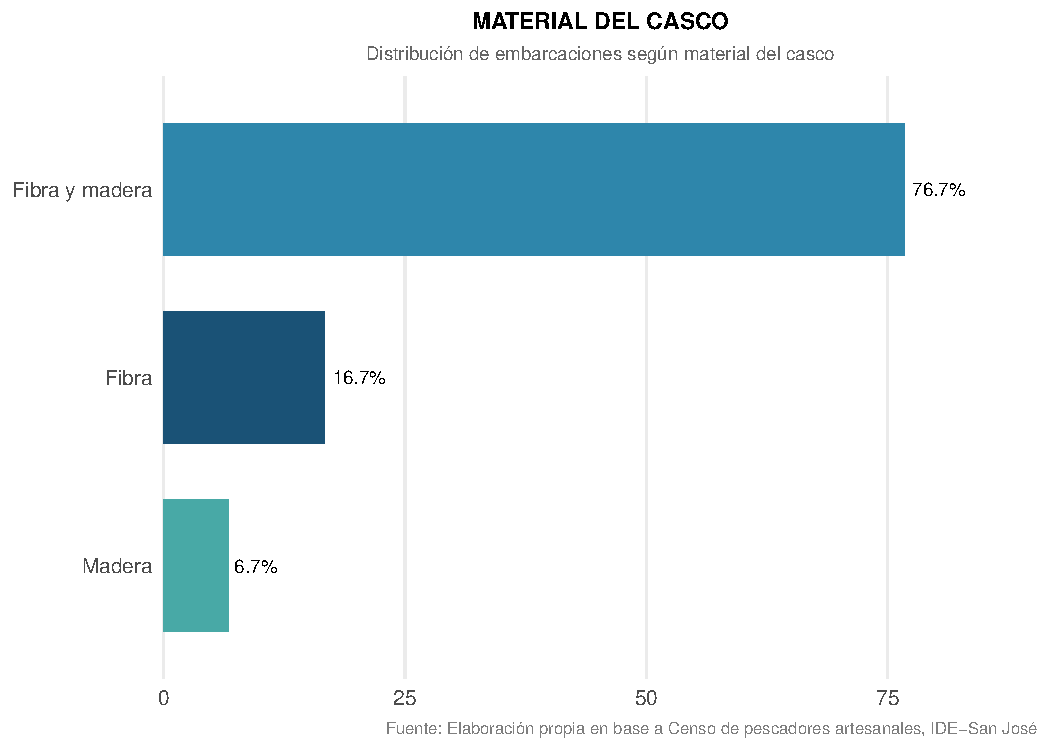
\includegraphics{analisis_pescadores_files/figure-pdf/unnamed-chunk-27-1.pdf}

\newpage

También se relevo sobre la percepción sobre el estado de las
embarcaciones.

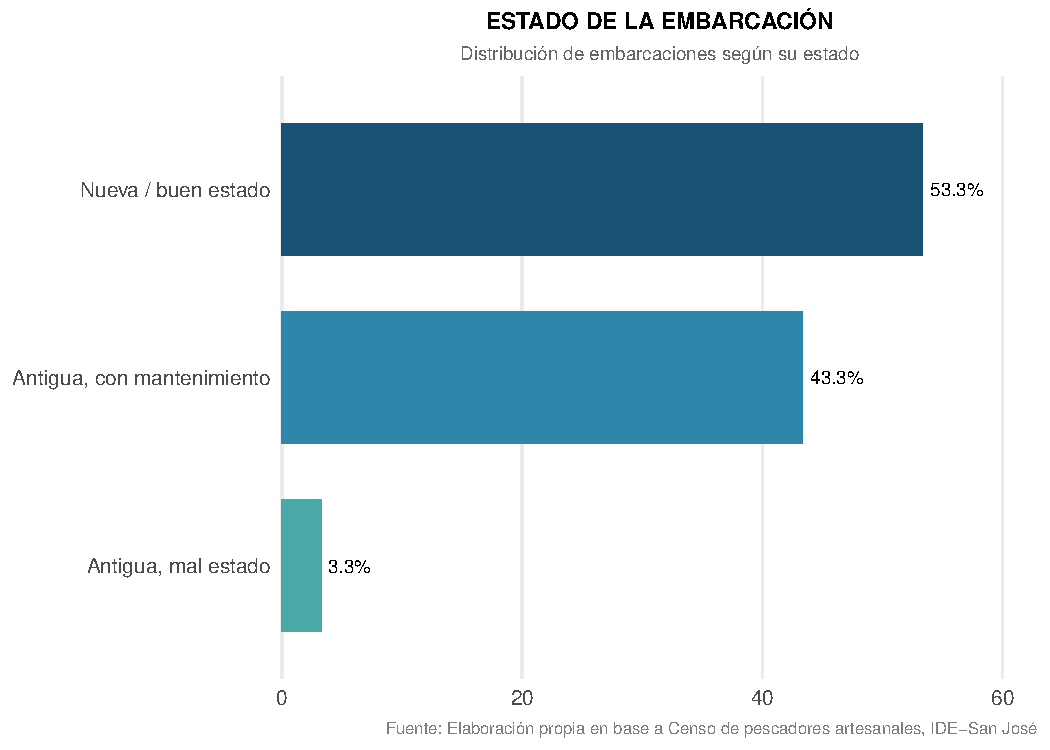
\includegraphics{analisis_pescadores_files/figure-pdf/unnamed-chunk-28-1.pdf}

Se informó que un 53\% de las embarcaciones son nueva o están en buen
estado; un 43\% si bien son antiguas, se encuentran en buen estado de
mantenimiento y un 3\%, además de antiguas, se están en mal estado.

En la tabla inferior se ve la distribución de las embarcaciones según
régimen de tenencia.

\begin{table}[H]
\centering
\caption{Tenencia de la embarcación}
\centering
\begin{tabular}[t]{l|c|c}
\hline
Tenencia & Cantidad & Porcentaje (\%)\\
\hline
Alquilada & 1 & 1.7\\
\hline
Compartida & 2 & 3.3\\
\hline
Propia & 57 & 95.0\\
\hline
\cellcolor[HTML]{f0f0f0}{\textbf{Total}} & \cellcolor[HTML]{f0f0f0}{\textbf{60}} & \cellcolor[HTML]{f0f0f0}{\textbf{100.0}}\\
\hline
\end{tabular}
\end{table}

Se observa que el 95\%, o sea 57 embarcaciones son propias; dos de
propiedad compartida y una es alquilada.

\newpage

Se consulto sobre el equipamiento de seguridad a bordo de las
embarcaciones.

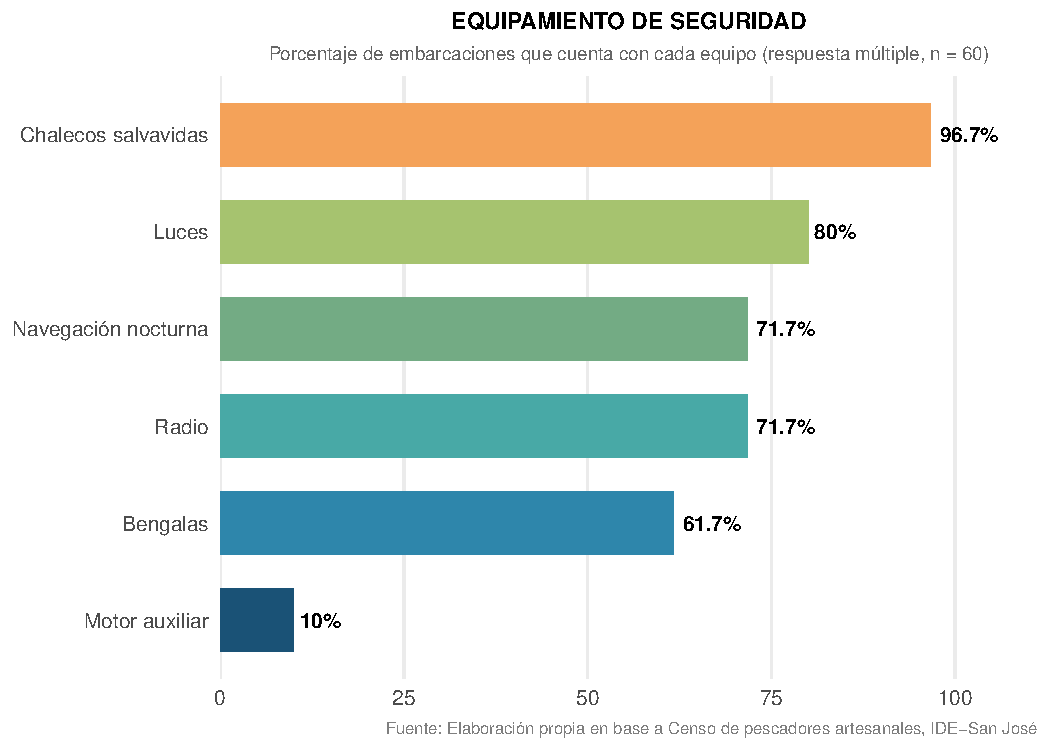
\includegraphics{analisis_pescadores_files/figure-pdf/unnamed-chunk-30-1.pdf}

Según la información aportada, el 97\% de las embarcaciones cuenta con
chalecos salvavidas; el 80\% tiene luces de navegación; un 72\% tiene
sistema de navegación; igual porcentaje tiene radio y un 62\% cuenta con
bengalas a bordo. Por último, un 10\% de las embarcaciones cuenta con
motor auxiliar.

\newpage

\hypertarget{formalizaciuxf3n-y-permisos}{%
\subsection{Formalización y
permisos}\label{formalizaciuxf3n-y-permisos}}

Se relevo sobre la situación de formalización y permisos de las
embarcaciones.

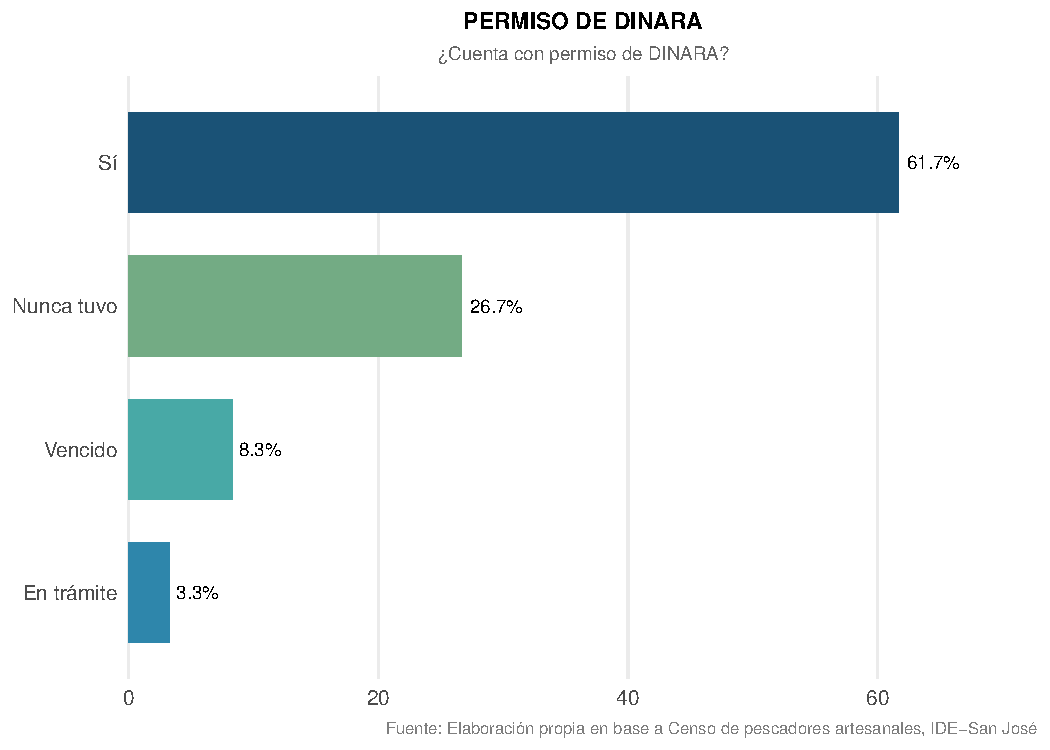
\includegraphics{analisis_pescadores_files/figure-pdf/unnamed-chunk-31-1.pdf}

En el gráfico superior, se ve que un 62\% de las embarcaciones cuentan
con el permiso de pescado de Dinara, mientras que un 38\% no lo tiene
aunque aquí se observan distintas situaciones: aquellas que nunca
tuvieron el permiso que representan el 27\% de las embarcaciones;
quienes lo tienen vencido, el 8\% y las embarcaciones que están con el
permiso en trámite, 3\%.

A aquellos que nunca tuvieron permiso (16) se les consultó si tienen
interés en formalizarse y el total de manifestó tenerlo.

\newpage

En cuanto a las dificultades que encuentran para formalizarse, tabla
inferior, un 45\% reclamó simplificar los trámites, un 30\% dijo que
estaban a la espera que Dinara habilitara el registro y una quinta parte
demanda asesoramiento e información.

\begin{table}[H]
\centering
\caption{Necesidades mencionadas para formalizarse}
\centering
\begin{tabular}[t]{l|c|c}
\hline
Tema & Cantidad & Porcentaje (\%)\\
\hline
Trámites y simplificación & 9 & 45\\
\hline
Permisos y cupos & 6 & 30\\
\hline
Información y asesoramiento & 4 & 20\\
\hline
Convocatoria / difusión & 1 & 5\\
\hline
\cellcolor[HTML]{f0f0f0}{\textbf{Total}} & \cellcolor[HTML]{f0f0f0}{\textbf{20}} & \cellcolor[HTML]{f0f0f0}{\textbf{100}}\\
\hline
\end{tabular}
\end{table}

En el gráfico inferior, se ve la distribución de las embarcaciones que
cuentan con permiso de Dinara y que tienen acceso a combustible con
descuento.

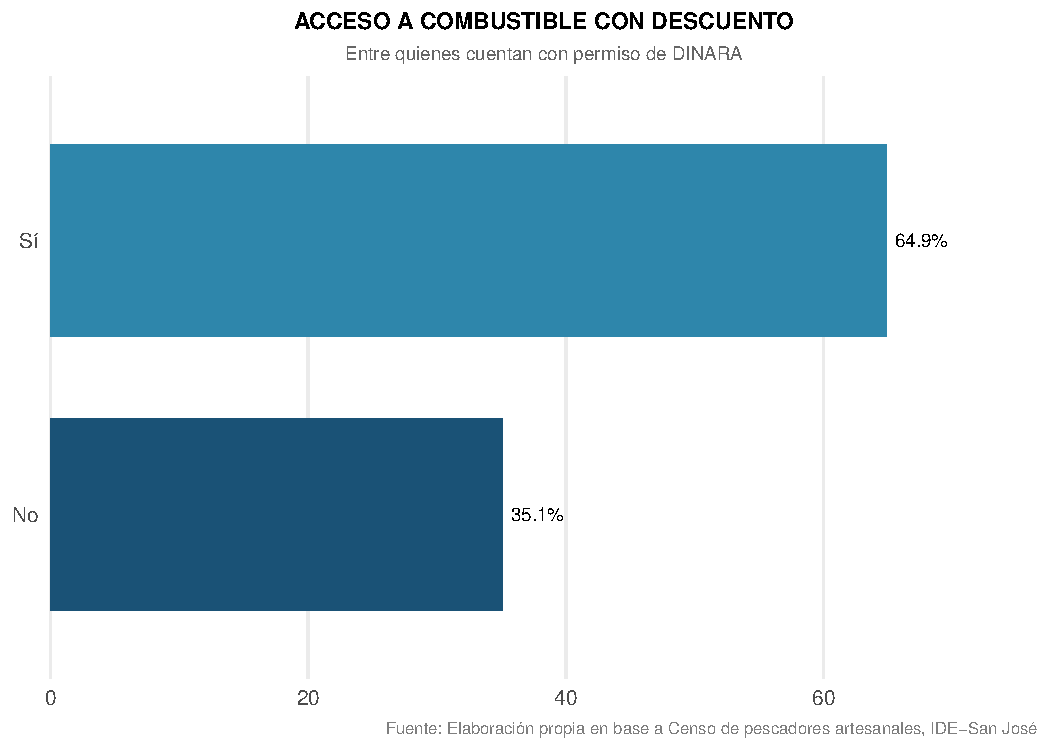
\includegraphics{analisis_pescadores_files/figure-pdf/unnamed-chunk-33-1.pdf}

El 35\% no acceden al beneficio y la razón queda expuesta en la página
siguiente en números absolutos y porcentajes.

\newpage

\begin{table}[H]
\centering
\caption{Motivo por el que no accede al descuento de combustible}
\centering
\begin{tabular}[t]{l|c|c}
\hline
Tema & Cantidad & Porcentaje (\%)\\
\hline
Trámite / documentación pendiente & 7 & 53.8\\
\hline
Situación con BPS & 3 & 23.1\\
\hline
Motivo económico / motor & 2 & 15.4\\
\hline
Desinterés & 1 & 7.7\\
\hline
\cellcolor[HTML]{f0f0f0}{\textbf{Total}} & \cellcolor[HTML]{f0f0f0}{\textbf{13}} & \cellcolor[HTML]{f0f0f0}{\textbf{100.0}}\\
\hline
\end{tabular}
\end{table}

Siete no acceden a combustible con descuento porque tienen trámites
pendientes que representan más del 50\%; tres por situación relativa con
el Banco de Previsión Social (BPS), dos por motivos económicos relativo
a la unidad de propulsión y uno por desinterés.

\newpage

Se preguntó también si regularmente reportaban a Dinara y Prefectura los
partes de pesca y despachos.

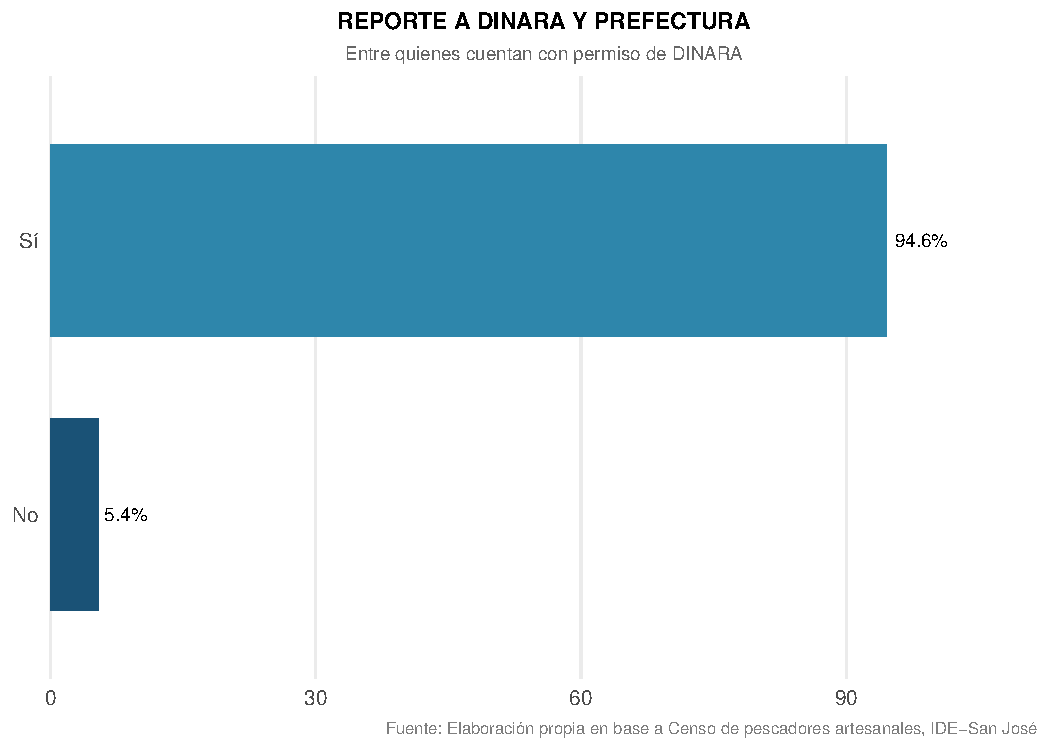
\includegraphics{analisis_pescadores_files/figure-pdf/unnamed-chunk-35-1.pdf}

Entre quienes cuentan con permiso de Dinara, el 95\% informaron que
reportaban cuando correspondía, mientras que el resto respondió
negativamente.

\newpage

\hypertarget{actividad-pesquera-zona-y-artes}{%
\subsection{Actividad pesquera: zona y
artes}\label{actividad-pesquera-zona-y-artes}}

La Dinara distribuye las zonas de pesca del Río de la Plata con una
codificación señalada con las letras D y E. Al departamento de San José
y parte de Colonia, le corresponde la letra D y a Montevideo y Canelones
la letra E.

\begin{figure}

{\centering 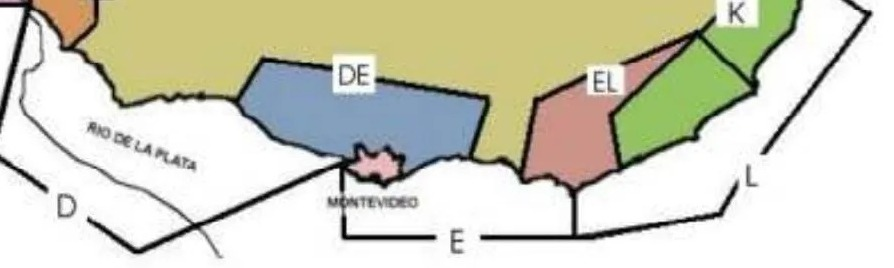
\includegraphics{zonas_pesca.jpeg}

}

\caption{Zonas de pesca establecidas por DINARA}

\end{figure}

Como se observa en la siguiente tabla, el 38\% de los pescadores tienen
habilitada la zona D, el 18\% las zonas D y E y un 5\% la zona E. Casi
la cuarta parte no brindó información al respecto.

\begin{table}[H]
\centering
\caption{Zona habilitada de pesca}
\centering
\begin{tabular}[t]{l|c|c}
\hline
Zona & Cantidad & Porcentaje (\%)\\
\hline
Sin dato & 23 & 38.3\\
\hline
Zona D & 23 & 38.3\\
\hline
Zona D y E & 11 & 18.3\\
\hline
Zona E & 3 & 5.0\\
\hline
\cellcolor[HTML]{f0f0f0}{\textbf{Total}} & \cellcolor[HTML]{f0f0f0}{\textbf{60}} & \cellcolor[HTML]{f0f0f0}{\textbf{100.0}}\\
\hline
\end{tabular}
\end{table}

\newpage

\hypertarget{artes}{%
\subsubsection{Artes}\label{artes}}

Se preguntó sobre el uso de artes de pesca. Los pescadores informaron
que el 100\% de las embarcaciones usa trasmallo; nueve de ellos (15\%)
usan además palangre y tres (5\%), utilizan línea de mano. Ninguno
informó usar otro tipo de artes. Entre quienes usan palangre la cantidad
de anzuelos utilizados va desde aquellos que solo cuentan decenas, la
mayoría, hasta dos embarcaciones que utilizan mil o más.

En el gráfico siguiente se informa sobre el largo total de las redes
utilizadas.

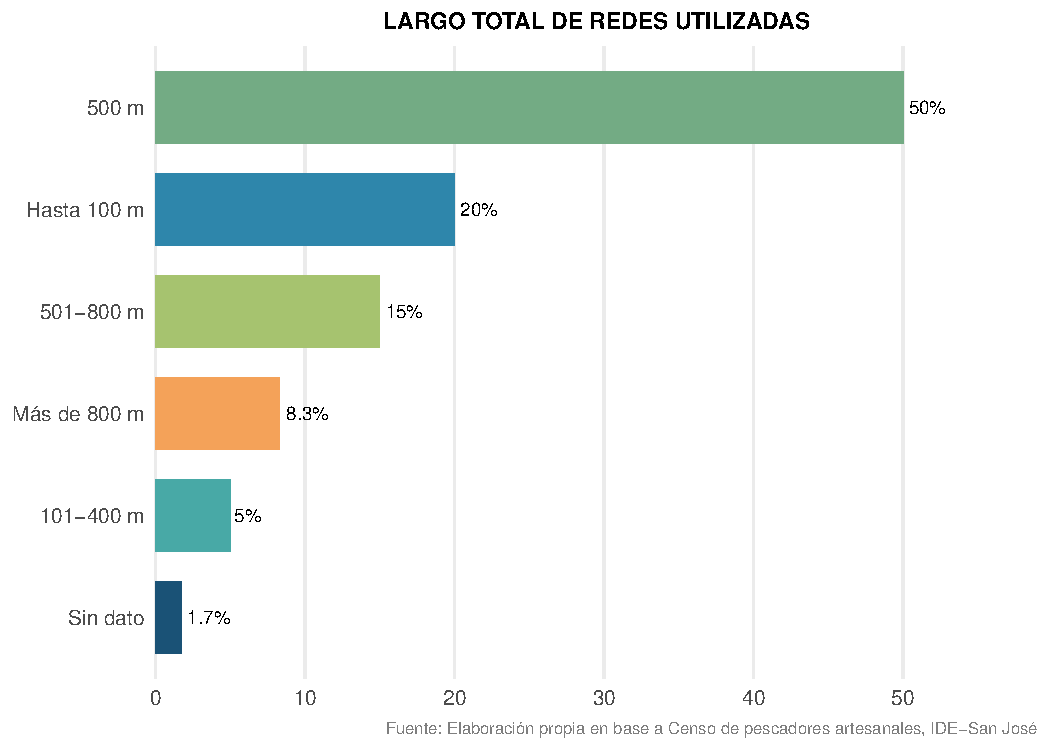
\includegraphics{analisis_pescadores_files/figure-pdf/unnamed-chunk-37-1.pdf}

La mitad de las embarcaciones usan un total de 500 metros de redes; un
15\% usan de 501 a 800 metros; un 8\% usan más de 800 metros de redes;
es decir, casi las tres cuartas partes usan 500 metros o más de redes.
Después se observa un 5\% que usan entre 101 metros y 400 y un 20\% que
usan 100 metros o menos.

\newpage

La distribución respecto a la luz de malla que usaban en sus redes fue
la siguiente:

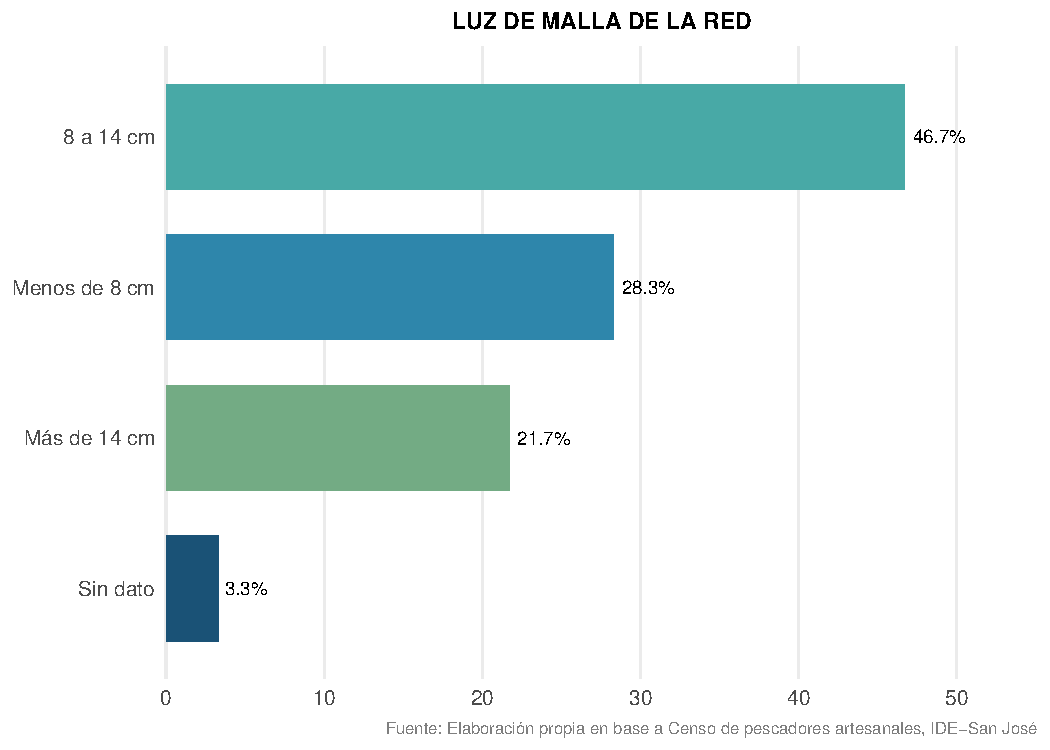
\includegraphics{analisis_pescadores_files/figure-pdf/unnamed-chunk-38-1.pdf}

Casi la mitad (un 47\%) dio usar redes con luz de malla de entre 8 y 14
centímetros; un 28\% luz de malla inferior a 8 cm; un 22\% más de 14 cm
y un 3\% no aportó información.

\newpage

\hypertarget{producciuxf3n-comercializaciuxf3n-y-descarte}{%
\subsection{Producción, comercialización y
descarte}\label{producciuxf3n-comercializaciuxf3n-y-descarte}}

En primer lugar se realiza una comparación sobre la producción en zafra
y fuera de zafra.

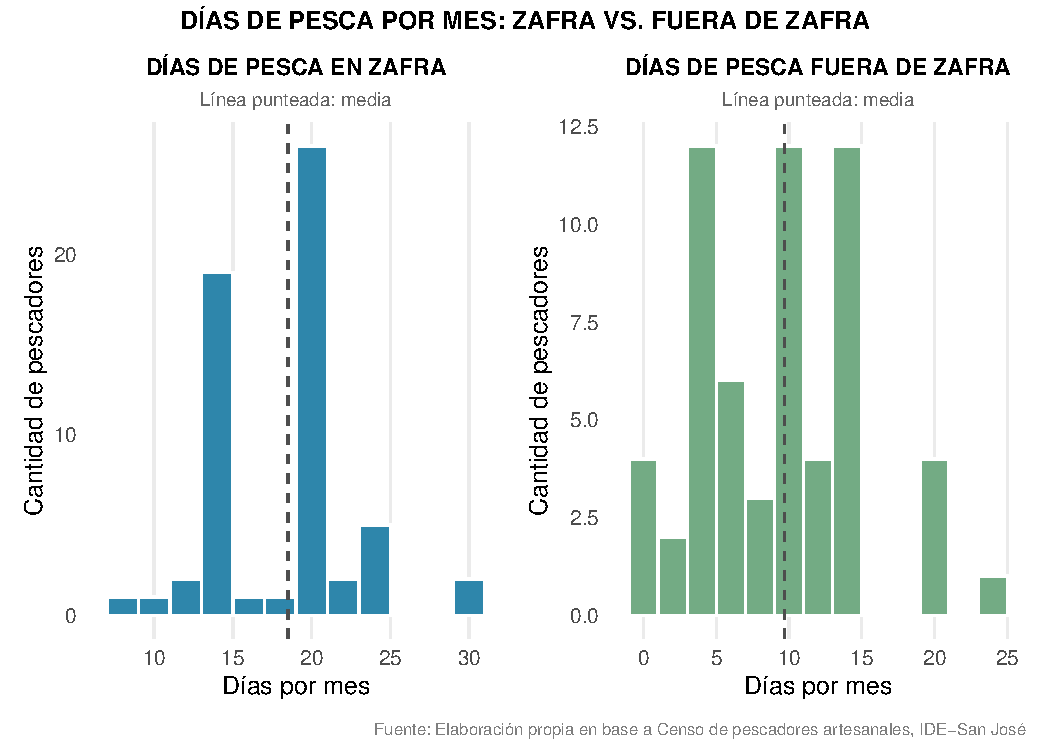
\includegraphics{analisis_pescadores_files/figure-pdf/unnamed-chunk-39-1.pdf}

La cantidad de días dedicados a la pesca muestra una marcada
estacionalidad. Durante la zafra, los pescadores trabajan en promedio 19
días al mes (mediana 20), lo que refleja una dedicación casi exclusiva a
la actividad. Fuera de zafra, el promedio cae a 9 días al mes (mediana
10), es decir, menos de la mitad. Esta diferencia es consistente con la
pluriactividad observada en otras variables: fuera de la zafra, los
pescadores combinan la pesca con otras actividades remuneradas (changas,
albañilería, trabajo rural) para sostener sus ingresos. La
estacionalidad, entonces, no solo afecta los ingresos mensuales ---como
se vio en la comparación de ganancias--- sino también la intensidad del
trabajo, configurando un ciclo anual de alta y baja dedicación.

\newpage

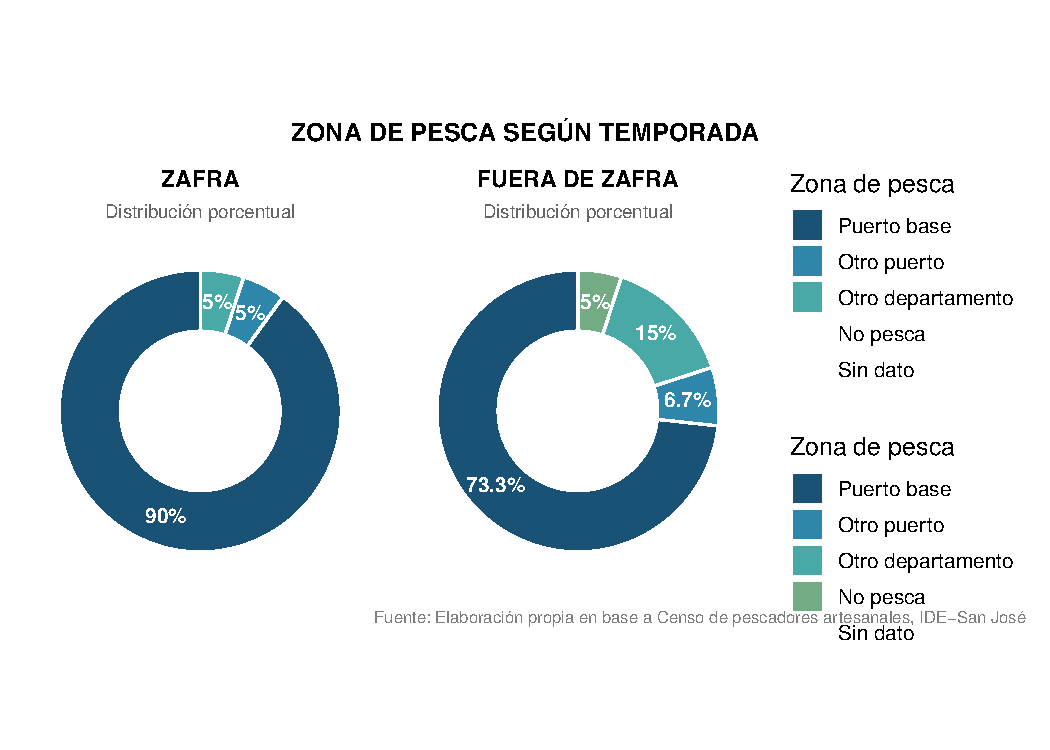
\includegraphics{analisis_pescadores_files/figure-pdf/unnamed-chunk-40-1.pdf}

Se observa una marcada diferencia en el radio de operación de la flota
según la temporada. Durante la zafra, la actividad es altamente
localizada: el 90\% de los pescadores opera exclusivamente en su puerto
base o localidad, y los traslados a otros puertos u otros departamentos
son marginales (5\% en cada caso). Sin embargo, fuera de zafra, la
dependencia del puerto base se reduce al 73,3\%. Esta caída se explica
por un fuerte aumento de la movilidad: un 15\% de los pescadores se
desplaza a operar en otros departamentos (el triple que en zafra) y un
6,7\% migra hacia otros puertos.En otro depto se menciona Colonia.

\newpage

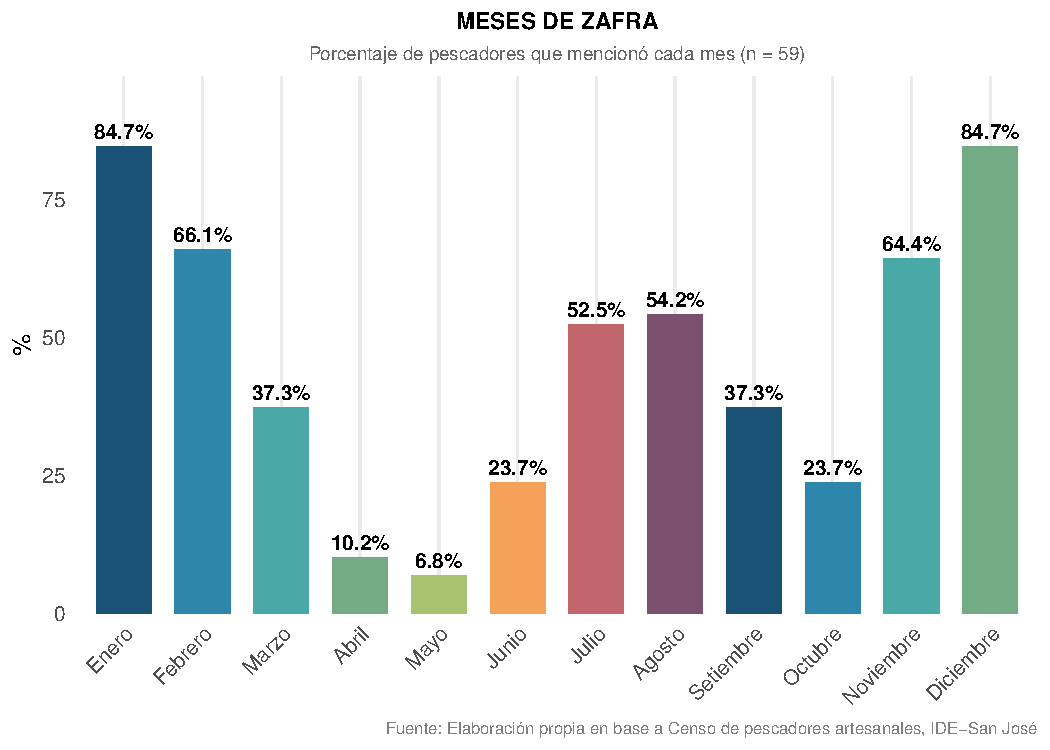
\includegraphics{analisis_pescadores_files/figure-pdf/unnamed-chunk-41-1.pdf}

La zafra de pesca en la zona no responde a un único bloque estacional,
sino que se distribuye en dos picos claros a lo largo del año. El
primero y más fuerte se da en el verano (diciembre a marzo), mientras
que el segundo se concentra en el invierno (julio y agosto). Los meses
de otoño (abril y mayo) son los de menor actividad. Esta bimodalidad
explica por qué los pescadores señalaban trabajar `todo el año': al
alternar entre la zafra de verano y la de invierno, logran mantener una
actividad relativamente constante, aunque con cambios en las especies
objetivo y en los volúmenes de captura.

\newpage

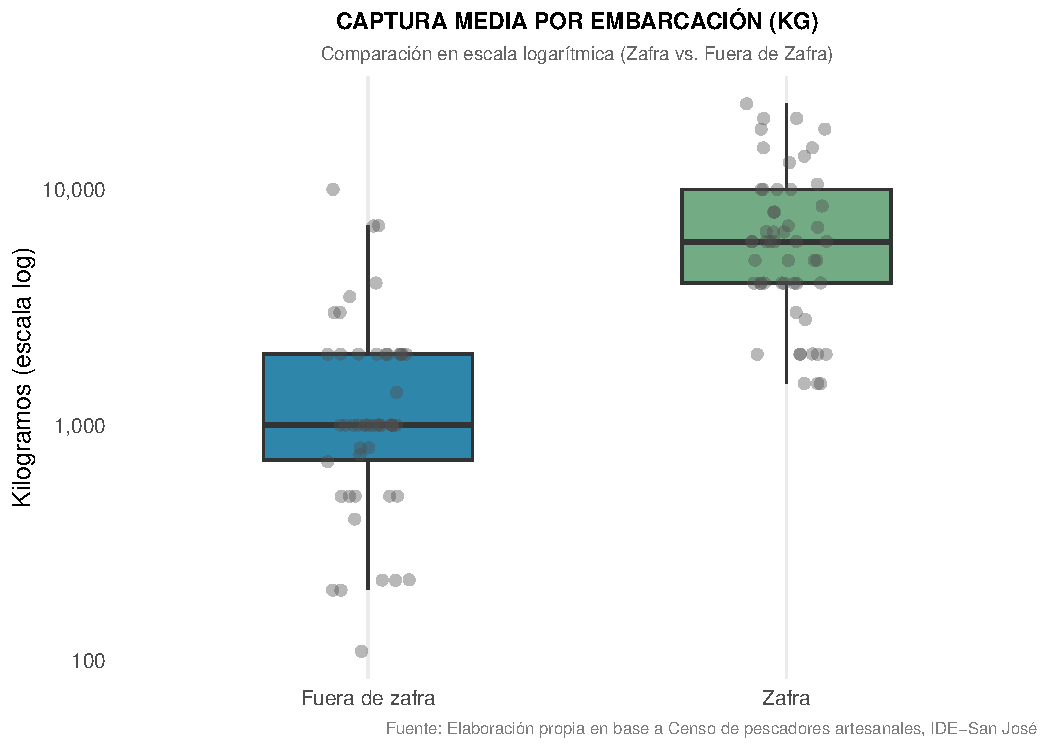
\includegraphics{analisis_pescadores_files/figure-pdf/unnamed-chunk-42-1.pdf}

El volumen de captura muestra una estacionalidad extrema. Mientras que
en zafra la mediana de captura es de 6.000 kg por embarcación, fuera de
zafra esta cifra cae abruptamente a 1.000 kg. Esta caída de más del 80\%
en el volumen extraído explica por qué los pescadores deben buscar otras
fuentes de ingreso o trabajar muchos menos días en los meses de veda.
Asimismo, la altísima dispersión (con casos que superan los 20.000 kg y
otros de apenas unos cientos) refleja una gran heterogeneidad en la
capacidad de pesca de la flota, probablemente asociada al tamaño de las
embarcaciones y a las artes de pesca utilizadas.

\newpage

A continuación se presentan datos sobre las especies más pescadas y el
destino de los descartes.

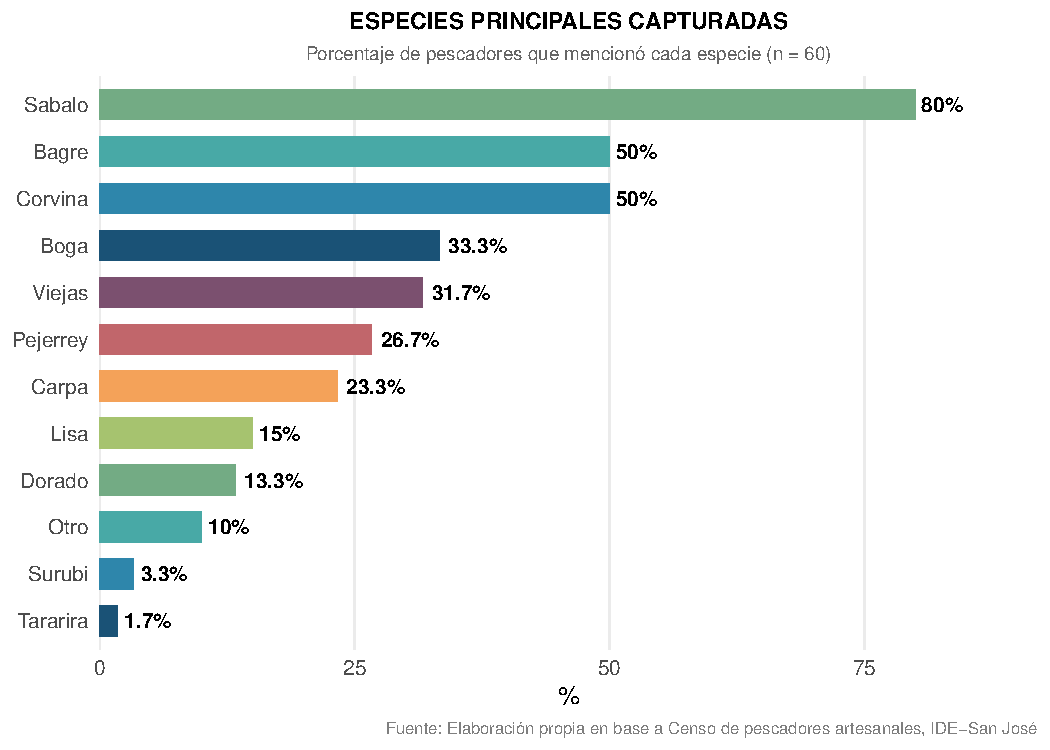
\includegraphics{analisis_pescadores_files/figure-pdf/unnamed-chunk-43-1.pdf}

La corvina, el sábalo y el bagre se posicionan como las especies
principales de la pesca artesanal en la zona, siendo mencionadas por la
gran mayoría de los pescadores. En un segundo plano aparecen especies
como la boga, viejas y el pejerrey, que dan cuenta de la diversidad de
la captura. Esta variedad refleja una estrategia de pesca
multiespecífica, característica del sector artesanal. Se registran cinco
casos que mencionan pescar especies no comercializables.

\newpage

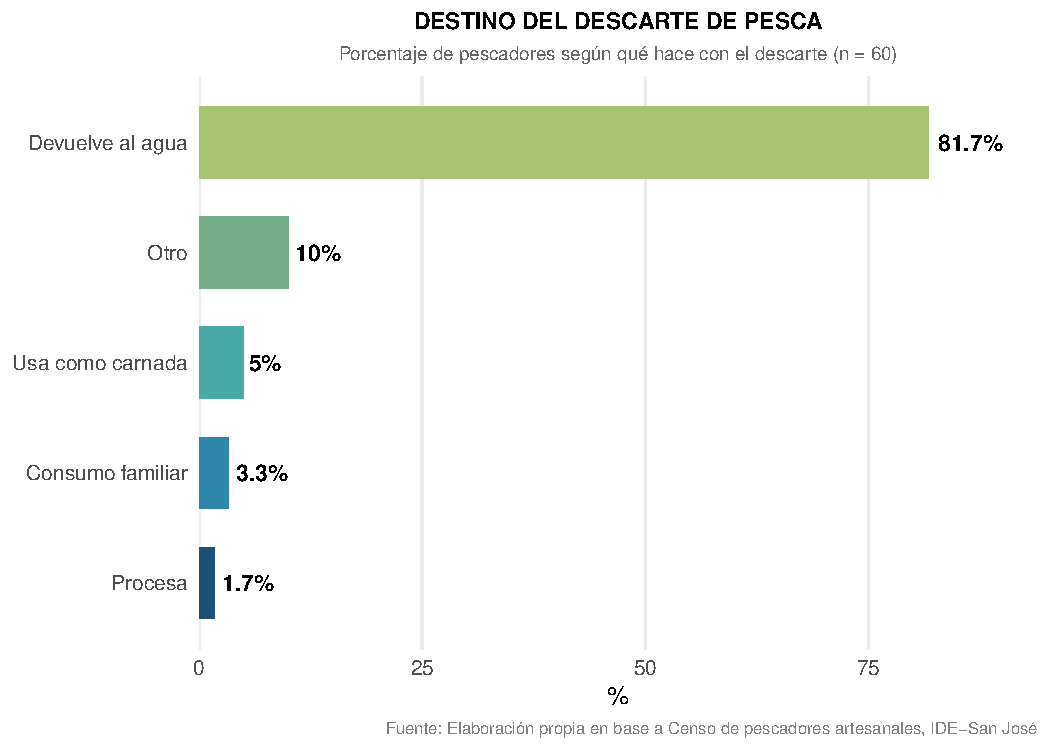
\includegraphics{analisis_pescadores_files/figure-pdf/unnamed-chunk-44-1.pdf}

El principal destino del descarte es la devolución al agua, una práctica
extendida entre casi todos los pescadores. En segundo lugar, y de forma
mucho más marginal, el descarte se reutiliza como carnada o se destina
al consumo familiar. La escasa presencia del procesamiento o la venta de
este excedente sugiere una oportunidad de mejora en la cadena de valor:
gran parte del volumen capturado y descartado podría tener un
aprovechamiento comercial o productivo que hoy se está perdiendo

\newpage

También se relevo información sobre la comercialización del producto.

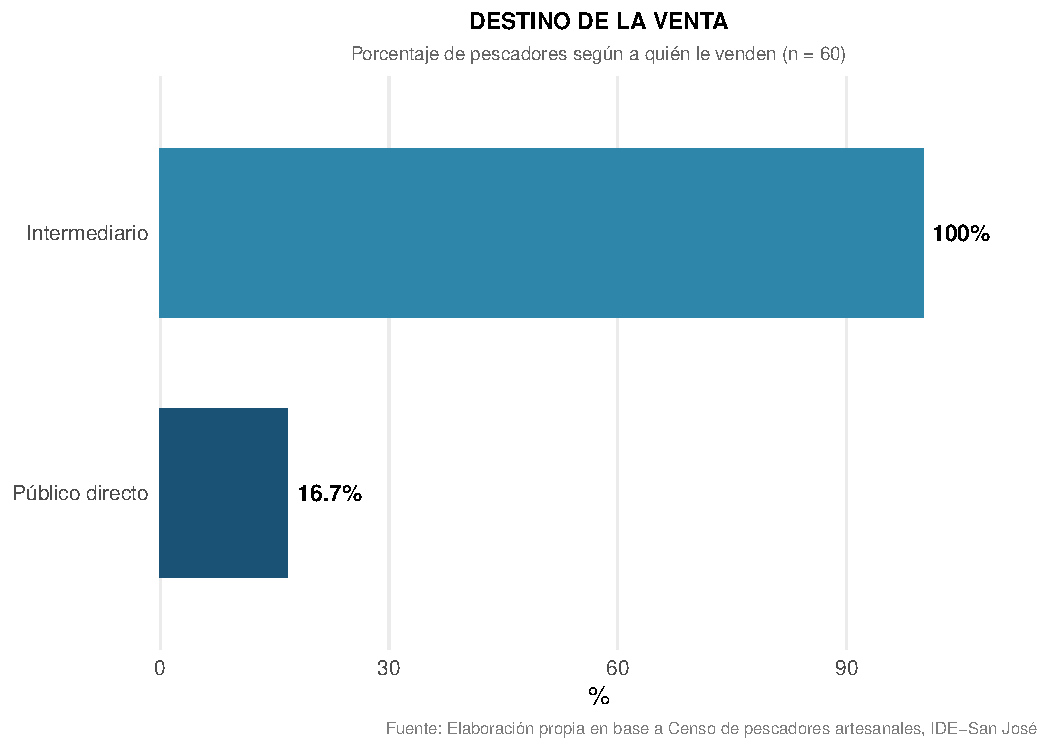
\includegraphics{analisis_pescadores_files/figure-pdf/unnamed-chunk-45-1.pdf}

La comercialización está dominada casi en su totalidad por la figura del
intermediario. Prácticamente el 100\% de los pescadores le vende a un
intermediario, y solo un pequeño porcentaje logra colocar parte de su
producción de forma directa al público. Esta estructura de
comercialización explica los reclamos por los `precios bajos' y el
`monopolio/oligopolio' mencionados en la sección anterior: el
intermediario captura el excedente del trabajo de los pescadores,
quienes tienen una capacidad de negociación muy limitada al no contar
con canales alternativos de venta

\newpage

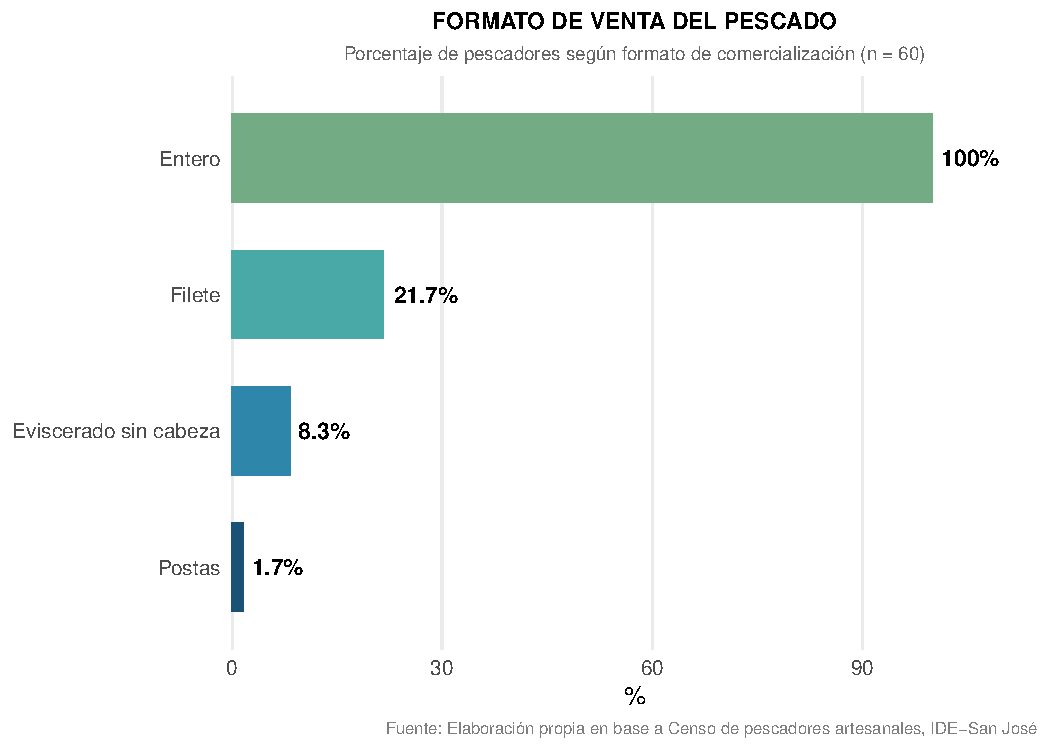
\includegraphics{analisis_pescadores_files/figure-pdf/unnamed-chunk-46-1.pdf}

La comercialización del pescado se realiza mayoritariamente en su
formato entero, lo que indica un bajo nivel de procesamiento o valor
agregado en origen. Un grupo menor, aunque significativo, comercializa
también en filete, eviscerado sin cabeza o en postas. Esto último
representa una oportunidad para fortalecer la cadena productiva local:
avanzar en la formalización de plantas de procesamiento o mesas de
fileteo permitiría a los pescadores capturar un mayor margen de
rentabilidad sobre su captura.

\newpage

Para terminar este apartado se preguntó sobre los precios de venta.

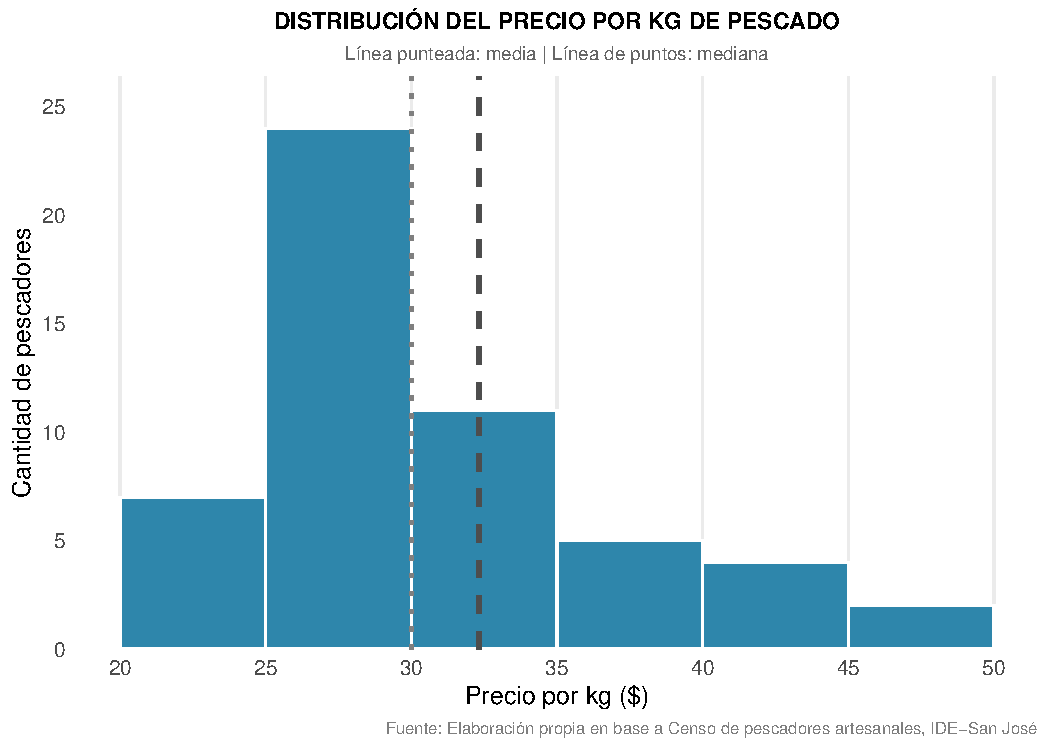
\includegraphics{analisis_pescadores_files/figure-pdf/unnamed-chunk-47-1.pdf}

El precio de venta del pescado por kilogramo presenta una alta
concentración en torno a los 30 pesos, siendo este el valor más
frecuente (la mediana). Sin embargo, se observa una importante
dispersión que va desde los 20 pesos hasta los 50 pesos por kg. Esta
variabilidad de precios para un mismo producto refleja la falta de un
precio de referencia estable y la vulnerabilidad de los pescadores
frente a los intermediarios (como se desprende de las entrevistas). La
moda en 30 pesos indica que, a pesar de los reclamos por `precios
bajos', la mayoría de las transacciones se realizan en un rango acotado
que muchas veces puede no cubrir los costos de salida.

\newpage

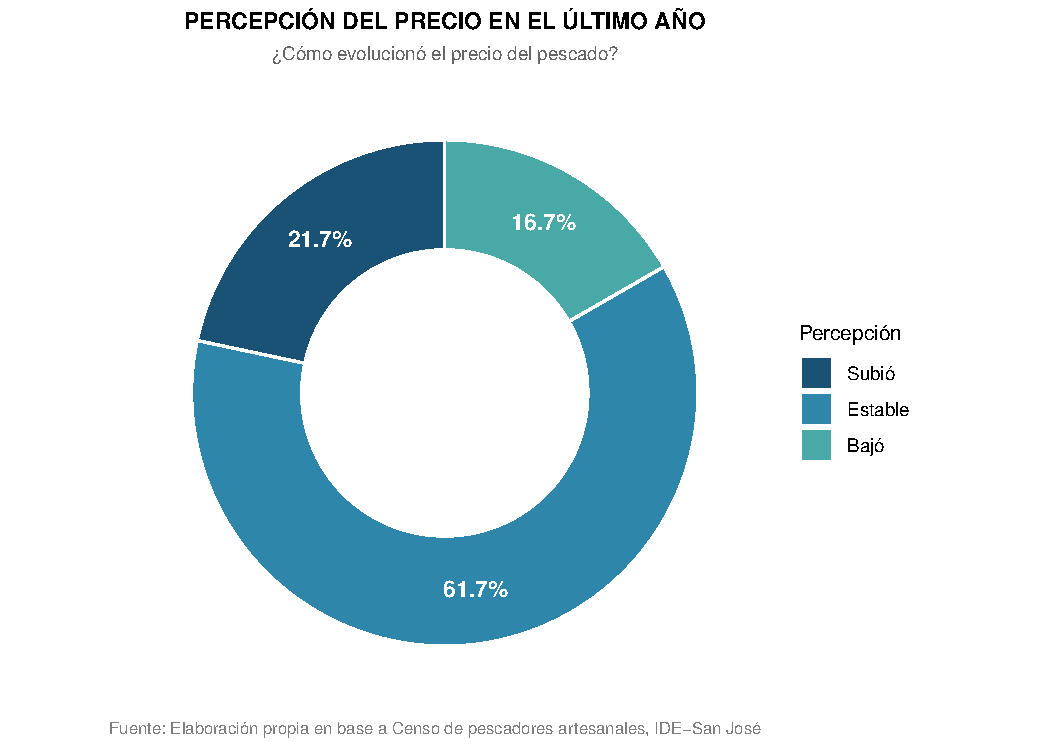
\includegraphics{analisis_pescadores_files/figure-pdf/unnamed-chunk-48-1.pdf}

Al consultar sobre la evolución del precio del pescado en el último año,
la mayoría de los pescadores percibe que el precio se mantuvo estable,
mientras que un grupo menor señala que subió o bajó. Esta percepción de
`estabilidad' es sumamente significativa si se la cruza con los datos de
inflación y aumento de costos: si el precio del pescado se mantuvo
estático (o subió por debajo de la inflación) mientras los costos
operativos (combustible, insumos, carnada) se incrementaron, el
resultado es una pérdida real de poder adquisitivo para el sector. Esto
dialoga directamente con la frase de un pescador en la sección
cualitativa: `Que seba, hace años se paga lo mismo'

\newpage

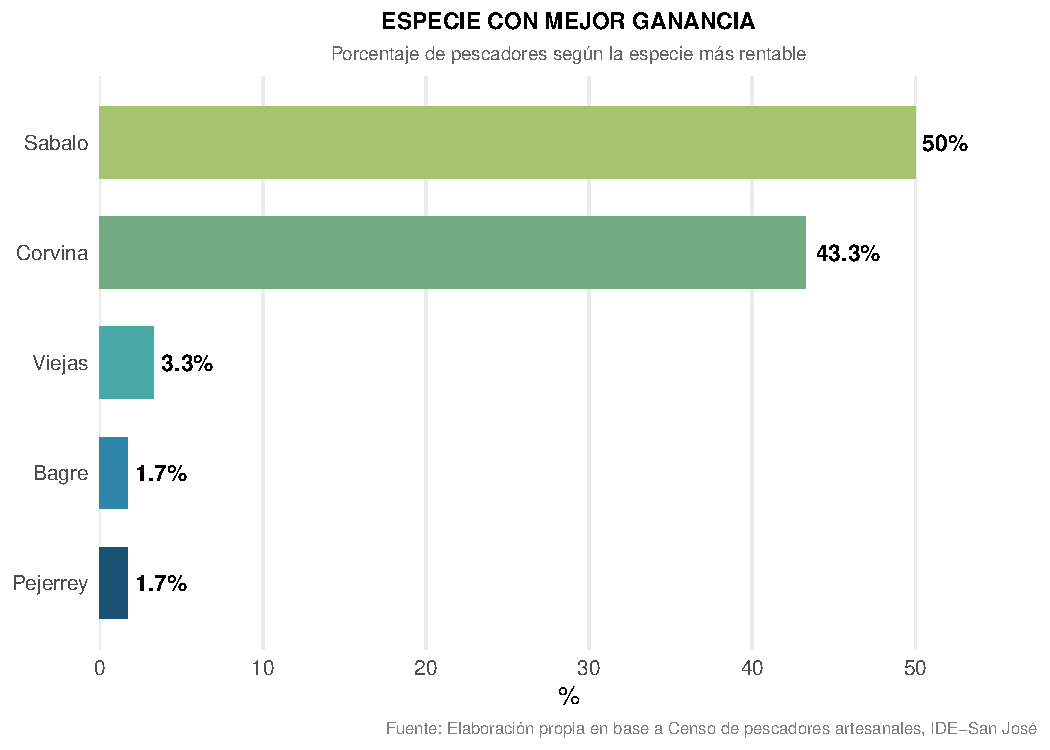
\includegraphics{analisis_pescadores_files/figure-pdf/unnamed-chunk-49-1.pdf}

Al consultar cuál es la especie que les reporta la mejor ganancia, las
respuestas se concentran casi exclusivamente en dos especies: el sábalo
y la corvina. El sábalo lidera las preferencias, lo que es coherente con
su alta presencia en las capturas y su demanda en el mercado. La
corvina, por su parte, ocupa un sólido segundo lugar. Esta concentración
en dos especies dominantes no solo refleja la biología del ecosistema,
sino también las estrategias comerciales de los pescadores: dependen de
muy pocas especies para sostener su rentabilidad, lo que los hace
altamente vulnerables a las fluctuaciones de precios, a la
sobreexplotación de esos recursos o a los cambios en la disponibilidad
estacional.

\newpage

\hypertarget{tripulaciuxf3n}{%
\subsection{Tripulación}\label{tripulaciuxf3n}}

Finalmente, se pregunto sobre la tripulación a bordo de las
embarcaciones y los desmalladores.

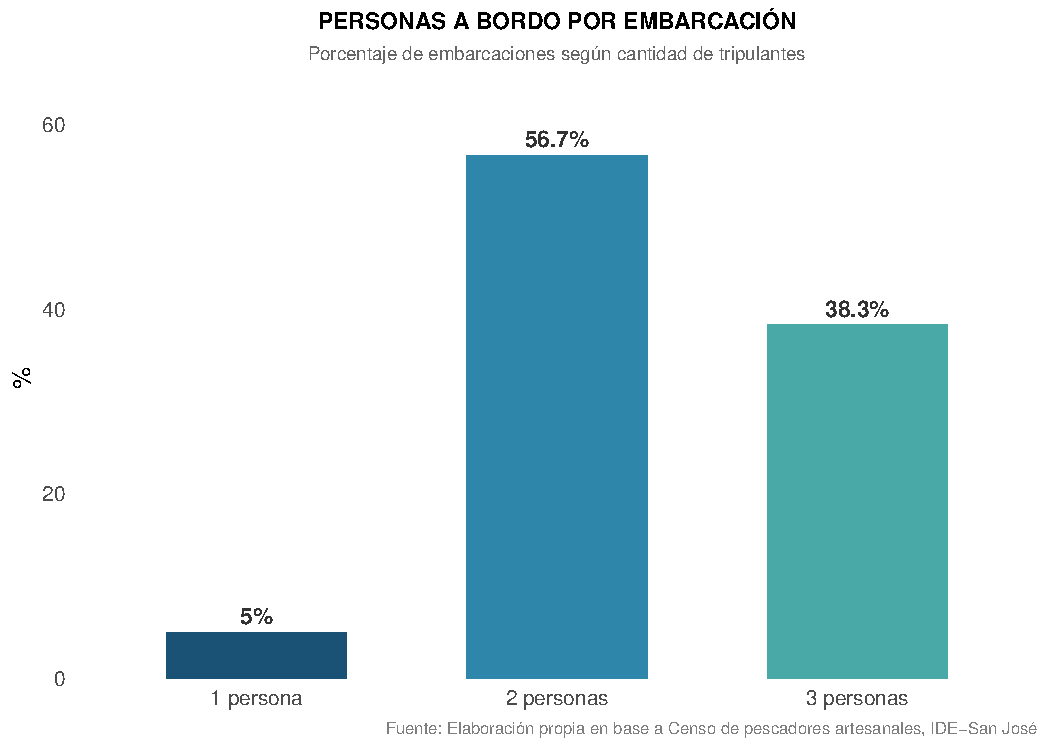
\includegraphics{analisis_pescadores_files/figure-pdf/unnamed-chunk-50-1.pdf}

La tripulación de la flota artesanal se caracteriza por ser reducida y
de tipo familiar o de dupla. Más de la mitad de las embarcaciones (un
56,7\%) opera habitualmente con 2 personas a bordo, mientras que un
38,3\% lo hace con 3 personas. Las salidas individuales (1 persona) son
prácticamente inexistentes, representando solo un 5\% de los casos. Esta
estructura de tripulación (predominio de dúos y tríos) es coherente con
la organización del trabajo artesanal: una persona se aboca a la
conducción de la embarcación y las artes de pesca, mientras que la otra
(u otras dos) colabora con la maniobra, la selección de la captura y el
desmallado. En total se registran 140 personas a bordo.

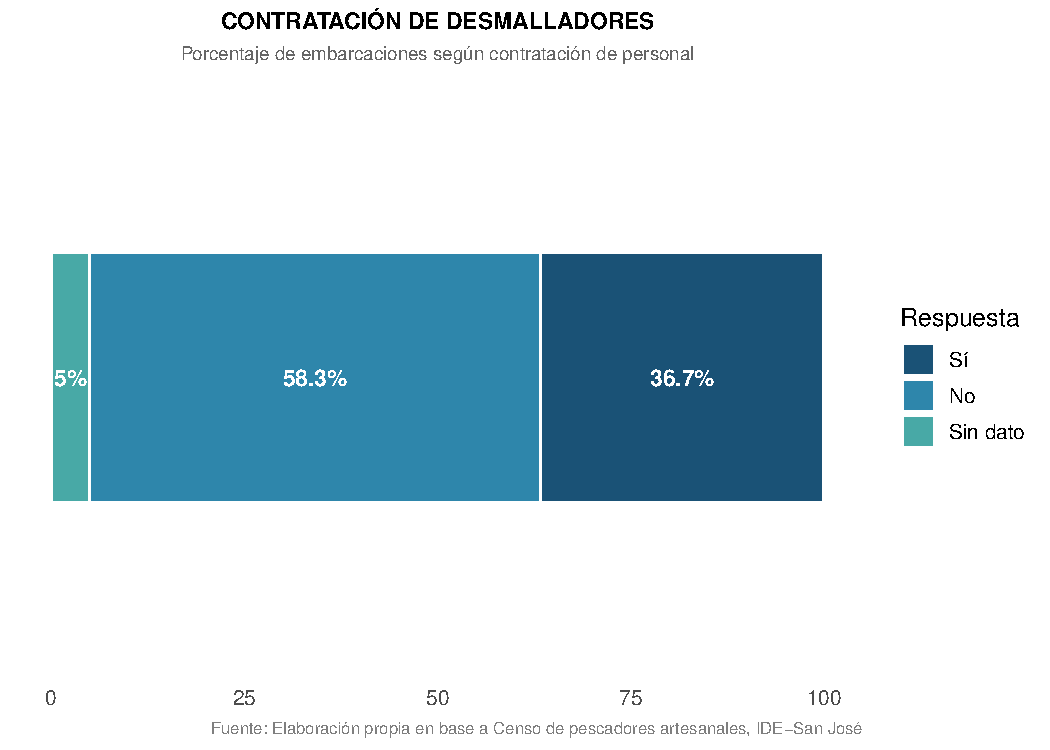
\includegraphics{analisis_pescadores_files/figure-pdf/unnamed-chunk-51-1.pdf}

Al consultar si la embarcación contrata desmalladores (personal
encargado de limpiar y preparar el pescado a bordo o en tierra), la
mayoría de los pescadores (cerca del 60\%) respondió que no contrata
este servicio. Esto refleja que el desmallado y la preparación del
pescado suelen ser tareas asumidas por los propios tripulantes de la
embarcación o por el núcleo familiar, antes que una actividad
tercerizada. La contratación de desmalladores queda restringida a un
poco más de un tercio de la flota, probablemente aquellas embarcaciones
de mayor porte o con volúmenes de captura más altos

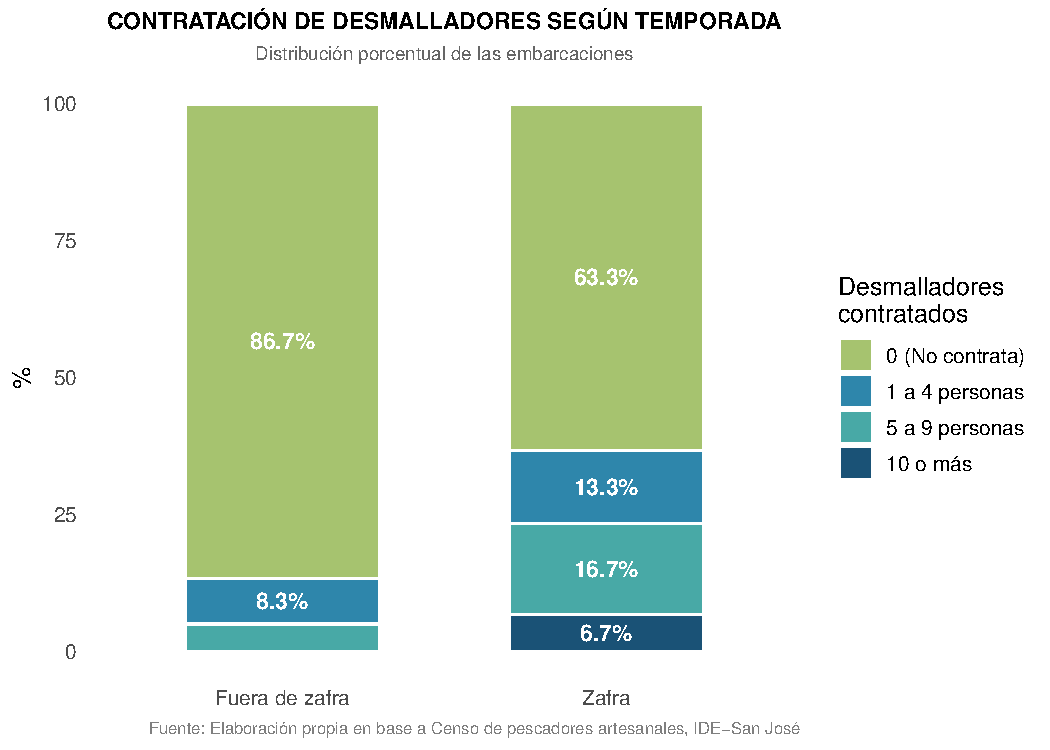
\includegraphics{analisis_pescadores_files/figure-pdf/unnamed-chunk-52-1.pdf}

La contratación de desmalladores presenta una fuerte estacionalidad
ligada a los volúmenes de captura. Durante la zafra, las embarcaciones
que tercerizan esta tarea contratan en promedio a 4 personas, llegando
en algunos casos a requerir hasta 20 trabajadores para el procesamiento
inicial del pescado. Sin embargo, fuera de la zafra, la mediana de
contratación cae a cero: la mayoría de las embarcaciones prescinde de
este personal, y quienes lo mantienen lo reducen a 1 o 2 personas. Esto
no solo confirma la caída de la actividad, sino que evidencia la
precarización del empleo en el sector: el trabajo de desmallado es un
empleo zafral por excelencia, que desaparece cuando baja la pesca

El volumen total de puestos de desmalladores contratados por la flota
cae drásticamente al finalizar la zafra. Mientras que en temporada de
zafra los pescadores suman un total de 113 contrataciones, fuera de
zafra ese número se desploma a apenas 28 personas.

Esto significa que, en los meses de baja actividad, desaparecen 85
puestos de trabajo vinculados directamente a la manipulación y
preparación del pescado, lo que representa una caída del 75\% en el
empleo de este rubro.

A nivel de cada embarcación, la diferencia también es notoria: el
promedio de desmalladores por barca pasa de 1,9 personas en zafra a solo
0,5 fuera de zafra. Esto confirma que el desmallado es una tarea
estrictamente zafral y que la gran mayoría de los tripulantes que se
dedican a esta función quedan sin trabajo en los meses de veda.

\hypertarget{conclusiones}{%
\chapter{Conclusiones}\label{conclusiones}}

1) Más del 60\% de los hogares y las personas que trabajan en la pesca
artesanal en el departamento ubican su lugar de residencia en la zona de
Arazatí y en el barrio Penino de Ciudad del Plata.

2) La mitad de los pescadores artesanales tienen una condición de
tenencia precaria de los terrenos donde residen, ubicándose la mayor
parte de estos en predios fiscales en calidad de ocupantes y otro grupo
en terrenos prestados.

3) En cuanto a la materialidad de las viviendas, casi un 40\% de los
hogares ocupan unidades con algún grado de precariedad.

4) Con relación a los servicios, se observa que aproximadamente una
cuarta parte de los pescadores artesanales no tiene acceso a agua segura
lo que se refleja en los reclamos registrados en formato cualitativo.
Con respecto a la evacuación de aguas servidas, más de las tres cuartas
parte vierte en pozo negro y casi una quinta parte de forma totalmente
precaria.

5) El sector tiene una significativa particpación en la actividad
productiva de mujeres, que representan más de la quinta parte de los
pescadores artesanales del departamento de San José. En relación a las
edades, dos tercios de pescadores/as tienen entre 25 y 55 años, siendo
el intervalo de mayor concentración entre 40 y 54 años.

6) Con respecto a nivel educativo, la actividad concentra trabajadores
cuya trayectoria en gran parte no supera los niveles iniciales de
educación formal: casi las tres cuarta parte de los pescadores dice
haber alcanzado Primaria. Si se le suma el primer ciclo de Educación
Secundaria se completa el 88\% de la población de estudio.

7) Se constata que se trata de un sector con significativa informalidad
en distintas dimensiones. Con relación a la previsión social, el 64\% no
realiza aportes al BPS. Con respecto a la actividad propiamente dicha,
alrededor de un 38\% no tiene permiso de Dinara y un 23\% de las
embarcaciones ingresa sin el permiso correspondiente de prefectura. Es
de destacar sí, que entre quienes nubnca han tenido permiso de Dinar, el
100\% manifiesta interés en regularizar.

8) Una quinta parte de los pescadores actualmente no están pudiendo
acceder al descuento de combustible que contempla al sector por una
variedad de situaciones explicitadas en el desarrollo del informe, lo
que les impide acceder a un beneficio importante para reducir costos
operativos. Ofrecer algún tipo de acompañamiento, podría facilitar la
regularización de algunos casos.

9) Al momento de identificar los principales problemas del sector,
cuatro aspectos aparecen como los más destacados: los bajos precios que
reciben por el producto, la formalización, dificultades de
infraestructura como ausencia y precariedad de muelle y la contaminación
que incide en los volúmenes de pesca.

10) Lo anterior es consistente con algunos de los interés manifestados
en materia de capacitación: comercialización y formalización. También se
recogió un significativo interés en capacitaciones relativas a la
seguridad náutica y manipulación del producto. .

\emph{(Por más consideraciones al respecto, léase los hallazgos de
carácter cualitativo en la página 29)}



\end{document}
